%!TEX root = ../../thesis.tex
\define{\chapterpath}{\allchapterspath/limitations}
\define{\imgpath}{\chapterpath/img}

%
\chapter{Limitations, Extensions and Derivatives}
\label{chapter:limitations}
\minitoc

Context - Why now: We have shown an algorithm that seems to work

Need - Why the reader: we need to know what are the hidden assumption that are really done and how to overcome them. And potential way to go into more complex problems

Task - Why me: I investigated this question and ran some proof of concept experiment that demonstrate my points.

Object - Why this chapter: We list a number of limitation (continuous state, finite set of task, pre-defined unique interaction frame, human is not affected by agent behavior). We then provide ideas to solve that problem and illustrate with some more or less toy example.

Findings - What: We found that there is some limitation and that some direction are shown to be working in simple scenarios.

Conclusions - So what: Let's go work on finding the limitation

Perspectives - What now: 


%%%%%%%%%%%%%%%%%%%%%%%%%%%%%%%%%%%%%%%%%%%%%%
%%%%%%%%%%%%%%%%%%%%%%%%%%%%%%%%%%%%%%%%%%%%%%
%%%%%%%%%%%%%%%%%%%%%%%%%%%%%%%%%%%%%%%%%%%%%%
%%%%%%%%%%%%%%%%%%%%%%%%%%%%%%%%%%%%%%%%%%%%%%
%%%%%%%%%%%%%%%%%%%%%%%%%%%%%%%%%%%%%%%%%%%%%%
%!TEX root = ../../thesis.tex

\section{Why should we temperate classifiers' predictions}
\label{chapter:limitiations:simplevsmatching}

We compare the performance of Equation~\ref{eq:matchingfilter} and Equation~\ref{eq:matchingfiltercrossvalidation} defined in chapter~\ref{chapter:lfui}. The main difference between these two equations is that the second (Equation~\ref{eq:matchingfiltercrossvalidation}) is adding another layer of verification, we temperate the prediction of the classifiers given our knowledge about their quality, which we measure by computing the confusion matrix via a cross-validation procedure.

\subsection{Artificial data}

We consider the same setting as for the experiments described in chapter~\ref{chapter:bci:EEGsignals} and used our two dimensional datasets of different qualities as presented in chapter~\ref{chapter:planning:artificialsignals}. We ran 500 simulations for each method. We consider only the planning method described in chapter~\ref{chapter:planning}.

\paragraph{Time to first task}  Figure~\ref{fig:timefirst_simplevsmatching} compares the number of iterations needed to reach the first task with confidence. We call the method using equation Equation~\ref{eq:matchingfilter} ``simple matching'' and we call ``matching'' the method using Equation~\ref{eq:matchingfiltercrossvalidation} which corrects the classifiers' predictions. There are strong differences between our methods especially for low quality datasets. For extremely overlapping data (50/60\% accuracy), the ``matching'' method is never confident about a task while the ``simple matching'' method show huge variability and sometime outputs confidence after very few time steps. 

\begin{figure}[!htbp]
\centering
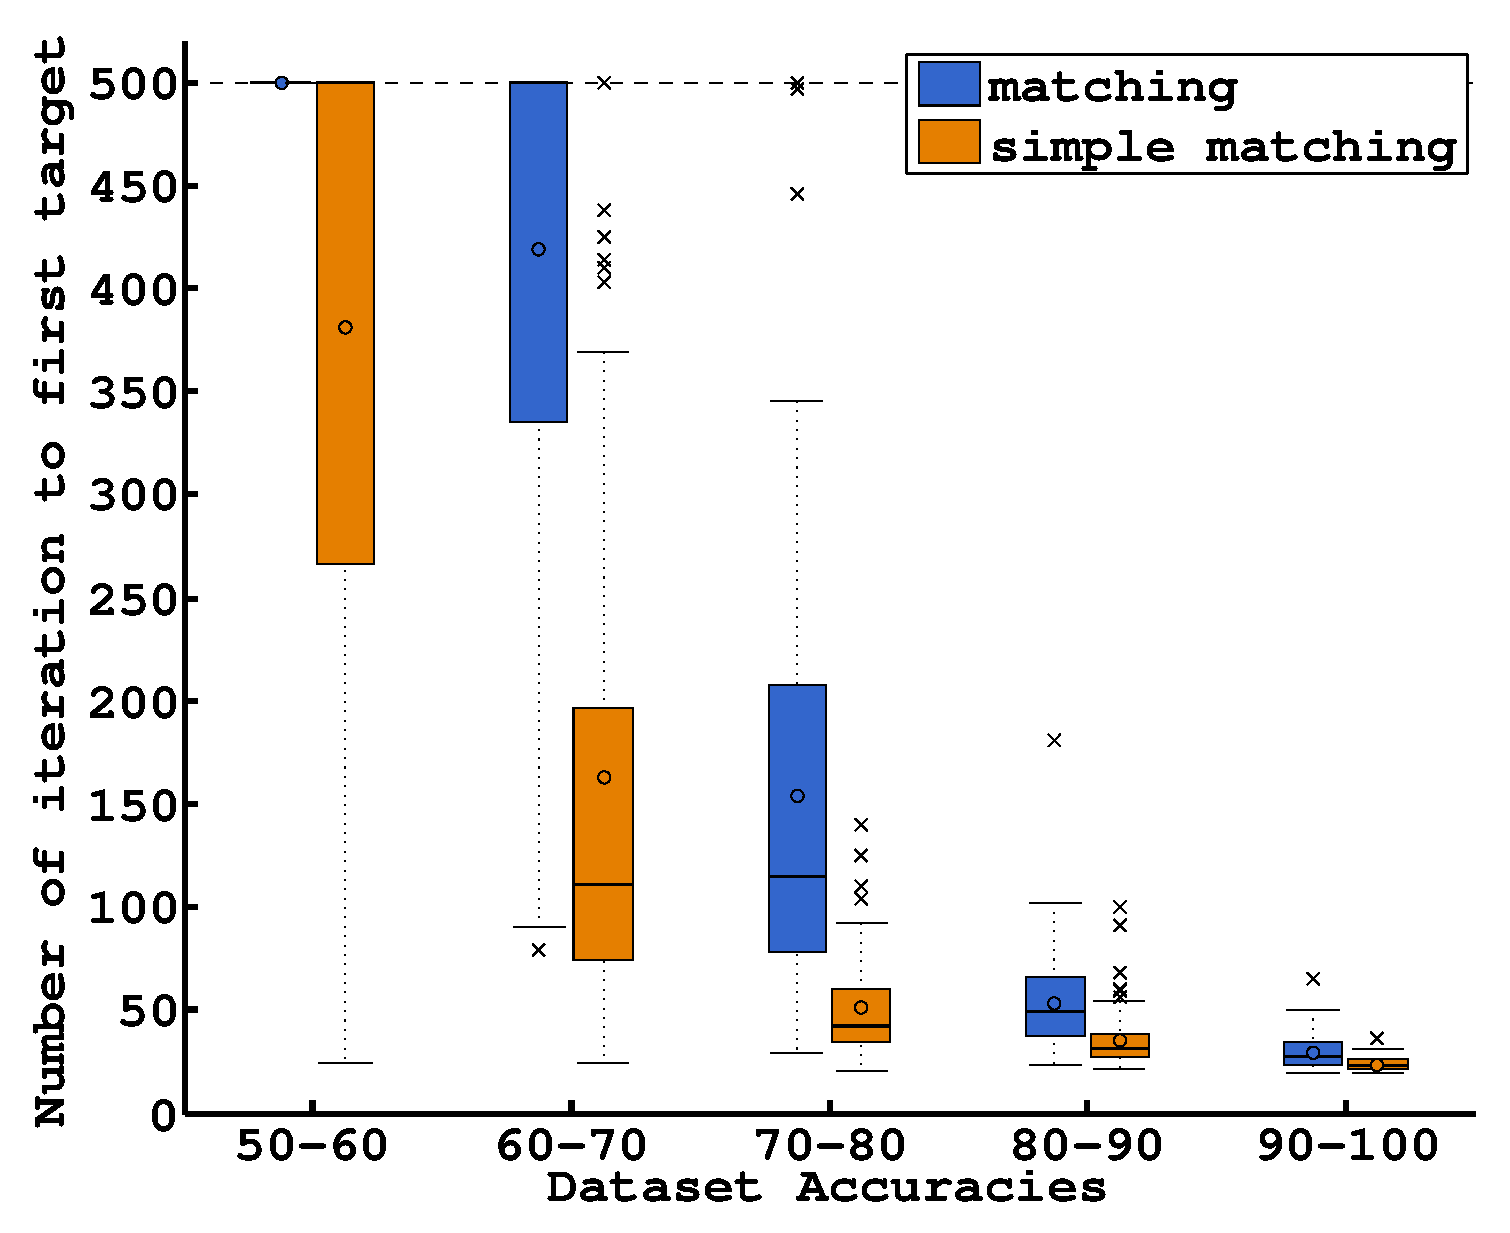
\includegraphics[width=\plotsize\columnwidth]{\imgpath/simplevsmatching/timefirst.eps}
\caption{Number of steps to complete the first task using 2D artificial datasets. Comparison between Equation~\ref{eq:matchingfilter} (simple matching) and Equation~\ref{eq:matchingfiltercrossvalidation} (matching), where the latter corrects the predictions of the classifiers given the estimation of their confusion matrix.}
\label{fig:timefirst_simplevsmatching}
\end{figure} 

This over confidence of the ``simple matching'' method reflects in the number of first tasks that were erroneously identified. As shown in Table~\ref{tab:errorTaskRatiosimplevsmatching}, the lower the quality of the data, the higher is the percentage of erroneously identified first task. For extremely overlapping data (50/60\% accuracy), this percentage goes up to 20 percent. While the ``matching'' method may seems too conservative, it is particularly important to not make mistakes when estimating the first task. Indeed once a first task is identified, its associated labels are taken as ground truth. A false estimation of the first task will falsify the signal-label pairs for the remaining of the interaction.

\begin{table}[!htbp]
\centering
\rowcolors{2}{gray!25}{white}
\begin{tabular}{c c c c}
    Dataset Accuracies & Simple Matching &  Matching \\ \hline
    50-60 & 0.21 & 0 \\ 
    60-70 & 0.16 & 0 \\
    70-80 & 0.03 & 0 \\
    80-90 & 0.02 & 0 \\
    90-100 & 0.01 & 0 \\
\end{tabular}
\caption{Percentage of time the estimation of the first task was erroneous using 2D artificial datasets. Comparison between Equation~\ref{eq:matchingfilter} (simple matching) and Equation~\ref{eq:matchingfiltercrossvalidation} (matching), where the latter corrects the predictions of the classifiers given the estimation of their confusion matrix. Only the ``matching'' method, which temperates the predictions of the classifiers, does not make mistakes when estimating the first task.}
\label{tab:errorTaskRatiosimplevsmatching}
\end{table}

\paragraph{Number of tasks achieved in 500 steps}

We compare the number of tasks correctly (Figure~\ref{fig:nCorrect_simplevsmatching}) and incorrectly (Figure~\ref{fig:nWrongEEG_simplevsmatching}) achieved in 500 steps between our two methods. While the ``simple matching'' method allows to reach more targets correctly, it also makes more mistakes for low quality datasets. The ``matching'' method is more conservative and does not make mistakes for all classifier quality, at the cost of reaching fewer targets.

\begin{figure}[!htbp]
\centering
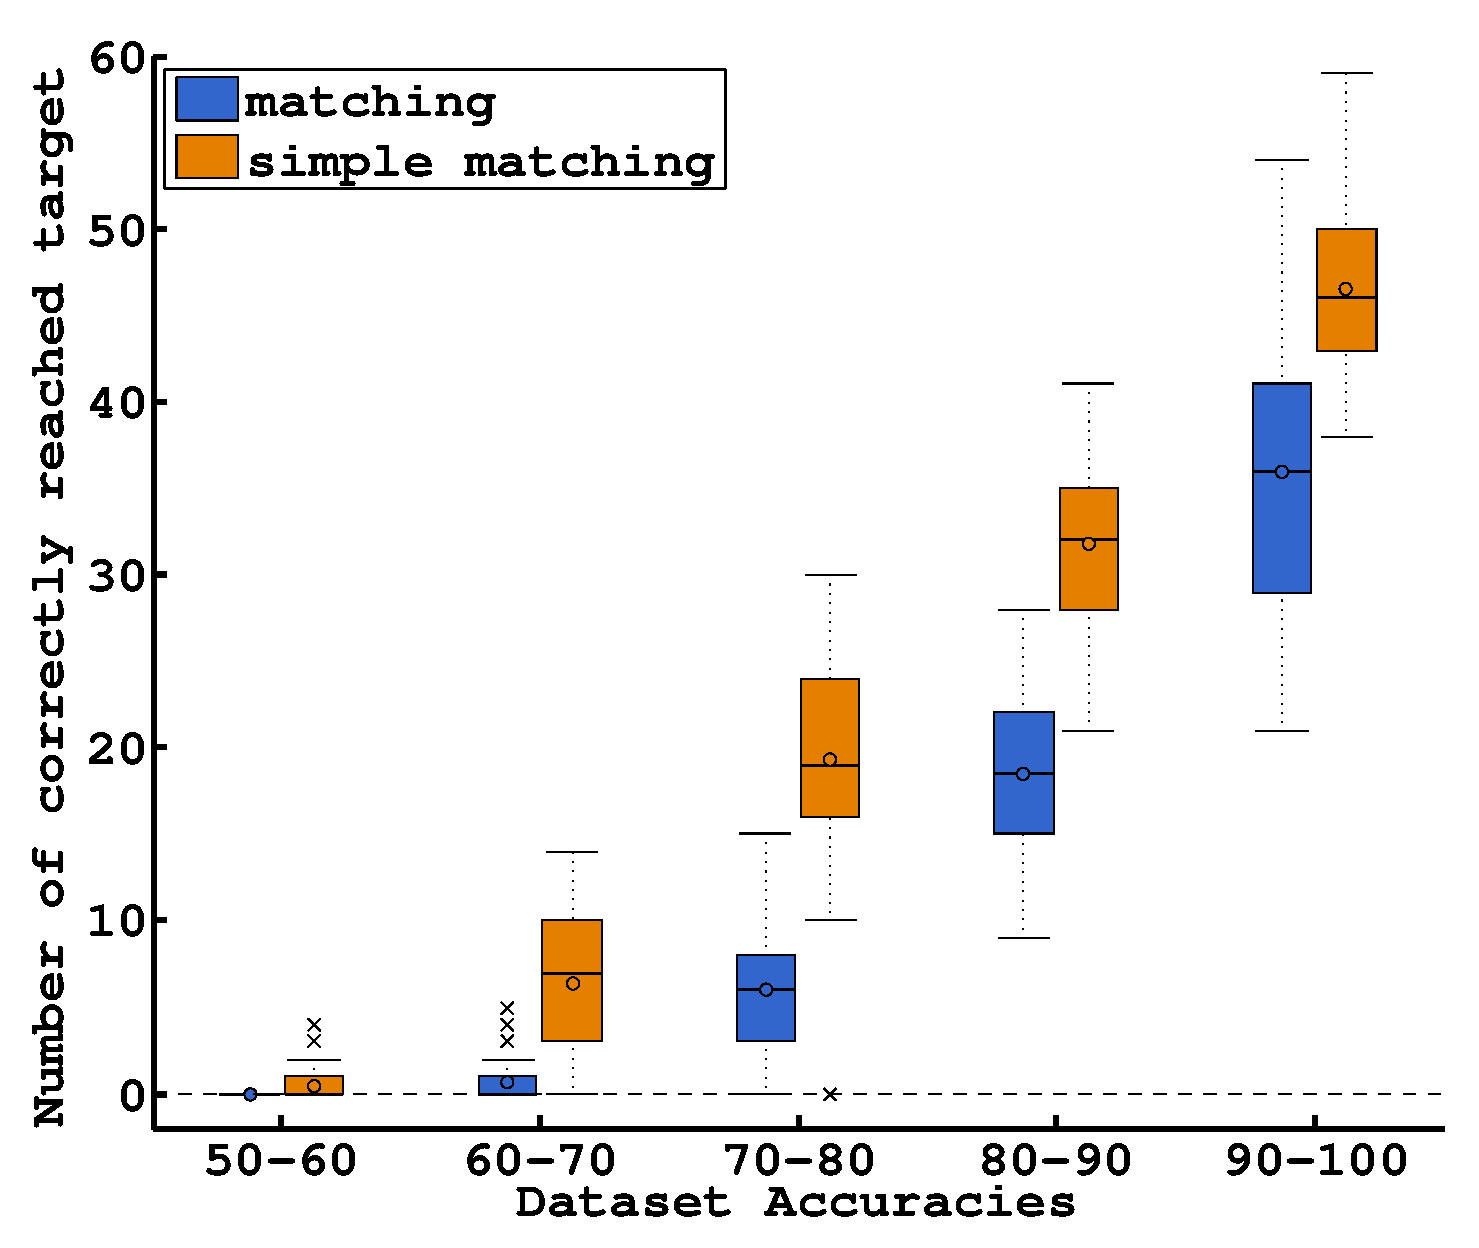
\includegraphics[width=\plotsize\columnwidth]{\imgpath/simplevsmatching/correct.eps}
\caption{Number of tasks correctly achieved in 500 steps using 2 dimensional artificial data. Comparison between Equation~\ref{eq:matchingfilter} (simple matching) and Equation~\ref{eq:matchingfiltercrossvalidation} (matching), where the latter corrects the predictions of the classifiers given the estimation of their confusion matrix. The ``simple matching'' method allows to reach more tasks correctly in 500 steps for all dataset quality.
}
\label{fig:nCorrect_simplevsmatching}
\end{figure} 

\begin{figure}[!htbp]
\centering
\includegraphics[width=\plotsize\columnwidth]{\imgpath/simplevsmatching/error.eps}
\caption{Number of tasks incorrectly achieved in 500 steps using 2 dimensional artificial data. Comparison between Equation~\ref{eq:matchingfilter} (simple matching) and Equation~\ref{eq:matchingfiltercrossvalidation} (matching), where the latter corrects the predictions of the classifiers given the estimation of their confusion matrix. The ``simple matching'' method starts making errors for dataset with accuracies lower than 80 percent. However, the ``matching'' method is more conservative and does not make mistakes.}
\label{fig:nWrongEEG_simplevsmatching}
\end{figure} 

\transition

These results considered only low dimensional dataset (2D), which were generated from Gaussian distribution matching perfectly with the assumption made by our classifiers. We now investigate how the performances are affected by more complex signals, such as the EEG datasets used in chapter~\ref{chapter:bci}, which are 34 dimensional with data distributions that do not necessarily follow the Gaussian assumption.

\subsection{EEG data}

We consider the same setting as for the previous subsection and use the EEG datasets described in chapter~\ref{chapter:bci}. We ran 500 simulations for each method. We consider only the active planning method used in chapter~\ref{chapter:planning}.

\paragraph{Time to first task} Figure~\ref{fig:timefirst_simplevsmatchingEEG} compares the number of iterations needed to reach the first task with confidence. There are strong differences between methods especially for low quality datasets. The ``simple matching'' method performances are not correlated with the classifiers' quality, which reflects the overconfidence of this method.

\begin{figure}[!htbp]
\centering
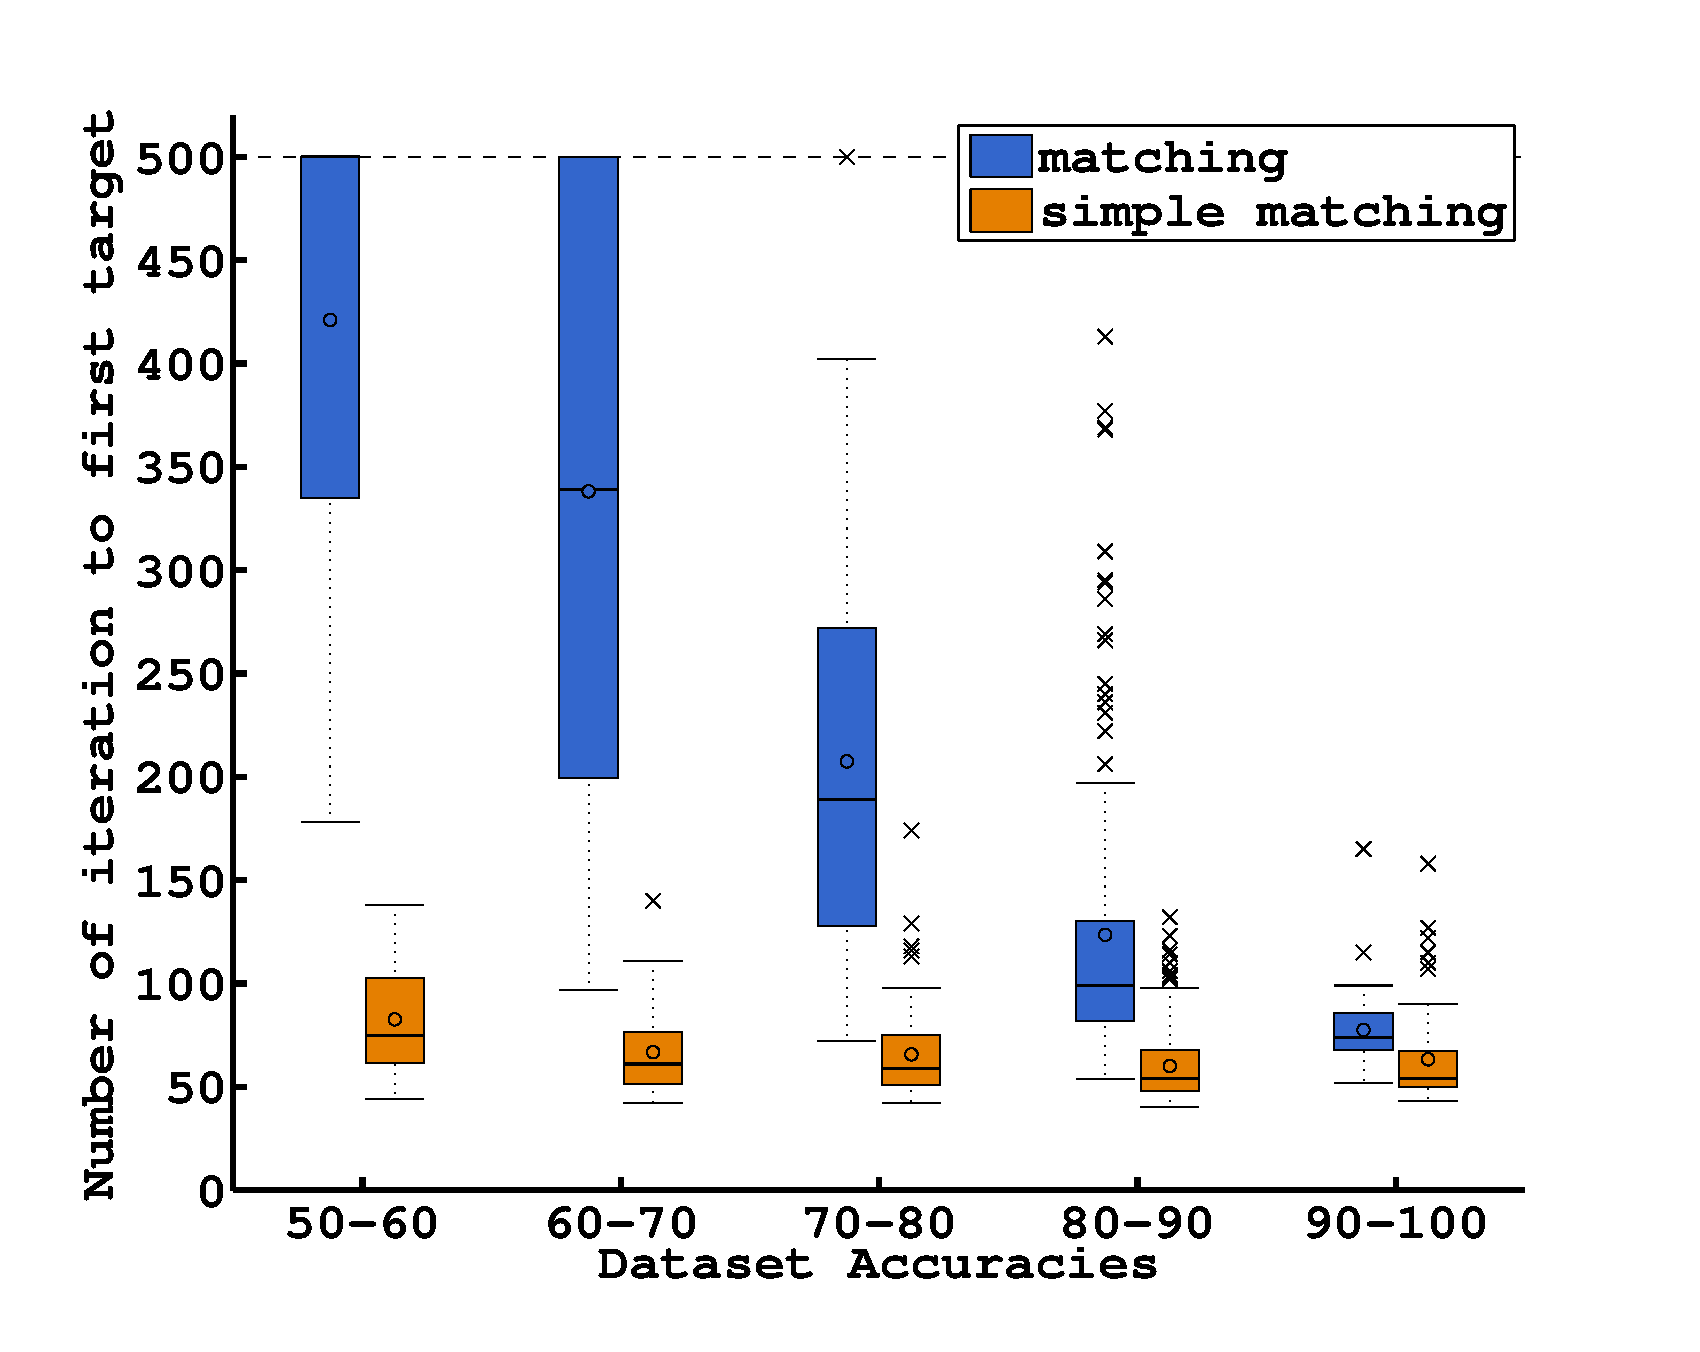
\includegraphics[width=\plotsize\columnwidth]{\imgpath/simplevsmatching/timefirstEEG.eps}
\caption{Number of steps to complete first task with our pre-recorded EEG data. Comparison between Equation~\ref{eq:matchingfilter} (simple matching) and Equation~\ref{eq:matchingfiltercrossvalidation} (matching), where the latter corrects the predictions of the classifiers given the estimation of their confusion matrix. The ``simple matching'' method performances are not correlated with the classifiers' quality, which reflects the overconfidence of this method.}
\label{fig:timefirst_simplevsmatchingEEG}
\end{figure} 

The over confidence of the ``simple matching'' method is reflected by the number of first tasks that were erroneously identified. As shown in Table~\ref{tab:errorTaskRatiosimplevsmatchingEEG}, the lower the quality of the data, the higher the percentage of erroneously identified first tasks. In all cases, this percentage was above 50 percent which makes the use of the ``simple matching'' method impossible for practical experiments. On the contrary, the ``matching'' method does not make any mistake when estimating the first task.

\begin{table}[!htbp]
\centering
\rowcolors{2}{gray!25}{white}
\begin{tabular}{c c c c}
    Dataset Accuracies & Simple Matching &  Matching \\ \hline
    50-60 & 0.81 & 0 \\ 
    60-70 & 0.80 & 0 \\
    70-80 & 0.66 & 0 \\
    80-90 & 0.53 & 0 \\
    90-100 & 0.60 & 0 \\
\end{tabular}
\caption{Percentage of time the first task estimation was erroneous using our pre-recorded EEG data. Comparison between Equation~\ref{eq:matchingfilter} (simple matching) and Equation~\ref{eq:matchingfiltercrossvalidation} (matching), where the latter corrects the predictions of the classifiers given the estimation of their confusion matrix. Only the ``matching'' method, that temperates the predictions of the classifiers does not make mistakes when estimating the first task.}
\label{tab:errorTaskRatiosimplevsmatchingEEG}
\end{table}

\paragraph{Number of tasks achieved in 500 steps}

We compare the number of task correctly (Figure~\ref{fig:nCorrect_simplevsmatchingEEG}) and incorrectly (Figure~\ref{fig:nWrongEEG_simplevsmatchingEEG}) reached in 500 steps. While the two methods allow to reach a similar number of targets correctly. The ``simple matching'' method also makes a many mistakes for all datasets. The ``matching'' method makes only few mistakes for all classifiers' quality.

\visuopti{\newpage}

\begin{figure}[!htbp]
\centering
\includegraphics[width=\plotsize\columnwidth]{\imgpath/simplevsmatching/correctEEG.eps}
\caption{Number of tasks correctly achieved in 500 steps using our pre-recorded EEG data. Comparison between Equation~\ref{eq:matchingfilter} (simple matching) and Equation~\ref{eq:matchingfiltercrossvalidation} (matching), where the latter corrects the predictions of the classifiers given the estimation of their confusion matrix. Both methods reach a similar number of targets correctly when using EEG datasets. The ``simple matching''  method shows more variability.}
\label{fig:nCorrect_simplevsmatchingEEG}
\end{figure} 

\begin{figure}[!htbp]
\centering
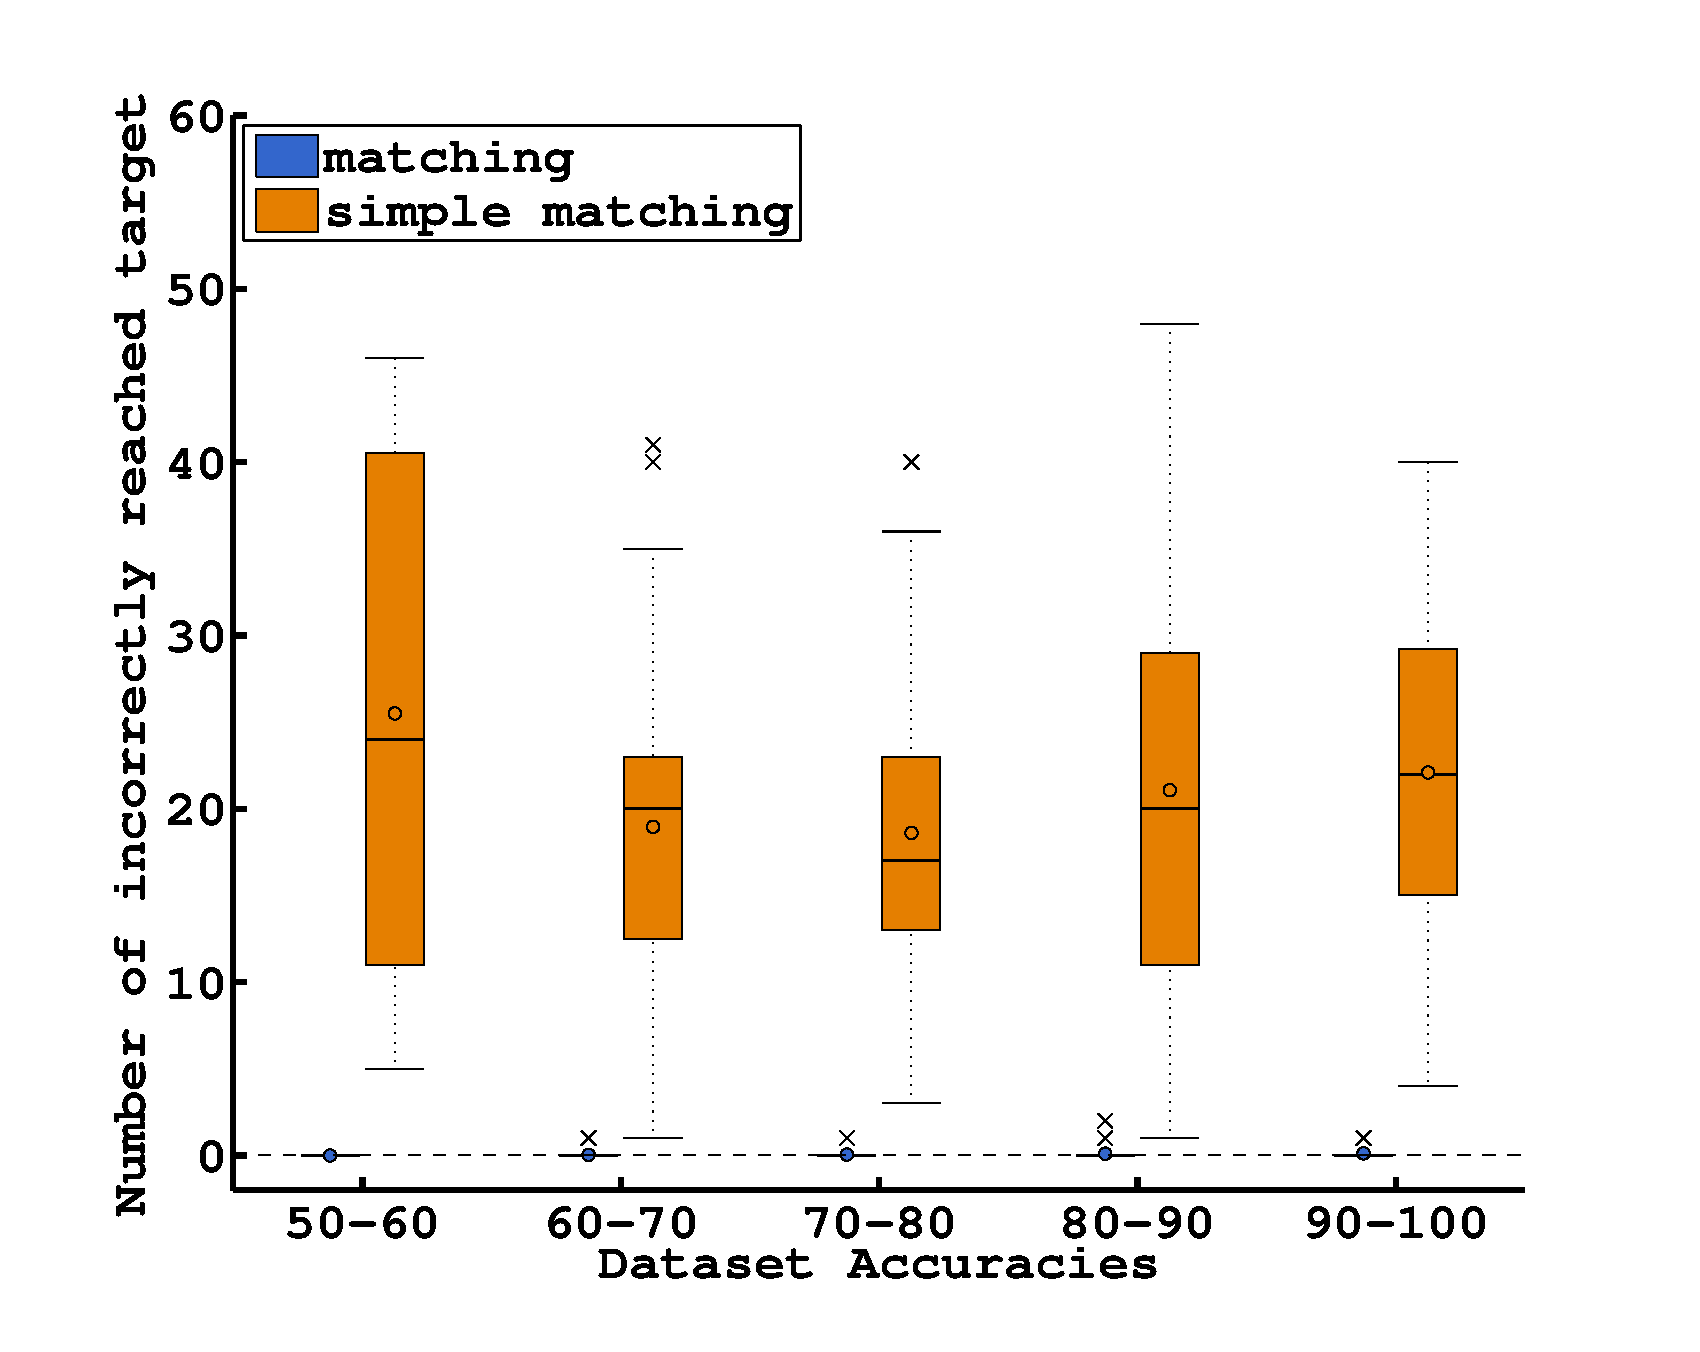
\includegraphics[width=\plotsize\columnwidth]{\imgpath/simplevsmatching/errorEEG.eps}
\caption{Number of tasks incorrectly achieved in 500 steps with our pre-recorded EEG data. Comparison between Equation~\ref{eq:matchingfilter} (simple matching) and Equation~\ref{eq:matchingfiltercrossvalidation} (matching), where the latter corrects the predictions of the classifiers given the estimation of their confusion matrix. The ``simple matching'' is not reliable for EEG data.}
\label{fig:nWrongEEG_simplevsmatchingEEG}
\end{figure} 

\subsection{Discussion}

The results presented in this section confirm that taking into account the uncertainty about the predictions of the classifiers makes the algorithm more robust. However, if we knew the data will be of good enough quality, it is not necessary to correct the classifiers' outputs (as we did for the speech dataset used in chapter~\ref{chapter:lfui}), which divides the computational cost by a factor of 10 (for a 10 fold cross-validation). However, as soon as we have to deal with signals of various qualities and with different properties (like for BCI data in chapter~\ref{chapter:bci}), it is better to include a measure of classification uncertainty in our likelihood update rule.


%%%%%%%%%%%%%%%%%%%%%%%%%%%%%%%%%%%%%%%%%%%%%%
%%%%%%%%%%%%%%%%%%%%%%%%%%%%%%%%%%%%%%%%%%%%%%
%%%%%%%%%%%%%%%%%%%%%%%%%%%%%%%%%%%%%%%%%%%%%%
%%%%%%%%%%%%%%%%%%%%%%%%%%%%%%%%%%%%%%%%%%%%%%
%%%%%%%%%%%%%%%%%%%%%%%%%%%%%%%%%%%%%%%%%%%%%%
%!TEX root = ../../thesis.tex

\section{Exploiting overlap between distributions}
\label{chapter:limitations:overlap}


In this section, we propose a method that uses the overlap between the model for each class to identify the correct task hypothesis, and demonstrate the efficiency of our uncertainty measure on the signal space presented in chapter~\ref{chapter:planning:uncertaintysignalspace}. We present simulated experiments using pre-recorded EEG signals, and show that we achieve similar performances than calibration based systems. Finally, we report online experiments where four users control, by means of a BCI, an agent on a virtual world to reach a target without any previous calibration process.

\subsection{Using the Bhattacharyya coefficient}

Following \cite{blankertz2010single}, we model the EEG signals using independent multivariate normal distributions for each class ($\mathcal{N}(\mu_c, \Sigma_c)$ and $\mathcal{N}(\mu_w, \Sigma_w)$). We will denote by $\theta$ this set of parameters $\{\mu_c, \Sigma_c,\mu_w, \Sigma_w\}$.

We propose to exploit the fact that when labels are mixed, the Gaussian corresponding to each classes should overlap more than for the correct label association (see Figure~\ref{fig:TworldLabelGaussian}). The Bhattacharyya coefficient measures this overlap, it has been related to the classification error of Gaussian models \cite{Kailath67} and is inversely proportional to the classification rate. Although there is no analytical relation between the coefficient and the classification rate, it is possible to derive bounds and good empirical approximations \cite{lee2000bayes}.

The Bhattacharyya coefficient $\rho \in [0,1]$ between the Gaussian distributions associated to label ``correct'' ($\mathcal{N}(\mu_c, \Sigma_c)$) and ``incorrect'' ($\mathcal{N}(\mu_w, \Sigma_w)$) is:

\begin{eqnarray}
\rho = e^{-D_B(\theta)}
\end{eqnarray}

where $D_B$ is the Bhattacharyya distance:

\begin{eqnarray}
D_B(\theta) = \frac{1}{8}(\mu_c-\mu_w)^T(\frac{\Sigma_c+\Sigma_w}{2})^{-1}(\mu_c-\mu_w)+\frac{1}{2}ln\left(\frac{det(\frac{\Sigma_c+\Sigma_w}{2})}{\sqrt{det\Sigma_c det\Sigma_w}}\right)
\end{eqnarray}

Finally, we approximate the expected classification rate as:
\begin{eqnarray}
Ecr \propto 1 - \rho
\end{eqnarray}

Now that we have an estimation of the expected classification rate, which is proportional to the overlap between the model of each class, we need to take a decision with respect to which task is the one intended by the user. To do so we compare the expected classification rate of every task hypothesis $\xi_t$ with $t \in \{1, \ldots, T\}$. 

The hypothesis whose associated model overlaps the less, i.e. which has the highest expected classification rate, i.e.\ the lowest value of $\rho$, is expected to be the one intended by the user. However it is meaningless to define an absolute threshold on the value of the expected classification rate itself. Indeed, different people generate different signals which result in classifiers of different qualities. Also, even the for the correct signal-label pairs, the model may overlap by quite some amount, as shown in our 2 dimensional examples in Figure~\ref{fig:datasetsquality}. To bypass this problem we rely on a voting system where we attribute to each hypothesis $\xi_t$ a weight that is updated at every iteration.

We rely on a pseudo-likelihood metric that for each hypothesis $\xi_t$ accumulates the expected classification rate over time:

\begin{eqnarray}
\L(\xi_t) = \prod_{i = 1}^{M} 1 - \rho_i^{\xi_t}
\end{eqnarray}
%
with $M$ the current number of iteration and $\rho_i^{\xi_t}$ the Bhattacharyya coefficient associated to task $\xi_t$ using all data up to time $i$. By normalizing the pseudo-likelihood values between every hypothesis, we obtain what can be viewed as the probability of each target:

\begin{eqnarray}
p(\xi_t) = \frac{\L(\xi_t)}{\sum_{u \in \{1, \ldots, T\}} \L(\xi_u)}
\end{eqnarray}

Once a target reaches a probability threshold $\beta$ we consider it as being the correct one, i.e.\ the one intended by the user. We used $\beta = 0.99$.

Finally, once we identified the first target, we will switch back to a classification based algorithm as described in chapter~\ref{chapter:lfui:tasttotask} and as used in the previous chapters of this thesis. We will see in section~\ref{chapter:limitations:overlap:offline} that this switch is necessary to maintain good performances since the classifier makes a much harder decision for each new EEG signal.

\subsection{Planning}

As we are using a model based method, we rely on our method measure that measure uncertainty directly in the signal space. This method was described in chapter~\ref{chapter:planning:uncertaintysignalspace} and to summarize rely on computing, for every state-action pairs, the similarity between the expected signals for each task. The more the expected signals are similar the less there is uncertainty.

For computing the similarity between two Gaussian distributions we could rely again on the Bhattacharyya coefficient describe above. However computing this coefficient between all models and for all state-action pairs was not feasible in real time. In order to improve computation efficiency we do not rely on a precise metric between Gaussian distributions and only consider the similarity between their means. The closest the means are, the more similar they are.

\subsection{Offline analysis}
\label{chapter:limitations:overlap:offline}

The objective of the offline analysis is to study the impact of our exploration method and evaluate if the classifier learned from scratch with our algorithm can be reused for learning new tasks. To ensure we have sufficient data to achieve statistically significant results, we rely on a large dataset of real EEG data. We used the same dataset as describe in chapter~\ref{chapter:bci:EEGsignals} dataset from \cite{iturrate2013task}, which covers ten subjects that performed two different control problems.

For each subject, we simulated 20 runs of 400 iterations following the control task. Each time the device performed an action, we sampled the dataset using the ground truth labels corresponding to the correct task and then removed the chosen signal from it. After a first task was identified we continued running the system to identify new tasks. 

We present most of the results in terms of the quality of the dataset, measured as the classification accuracy that a calibrated brain signal classifier would obtain.

\paragraph{Planning Methods}

We compared the average number of steps (with maximum values of 400 steps) needed to identify the first task when learning from scratch with different planning methods.

\begin{figure}[!ht]
    \centering
    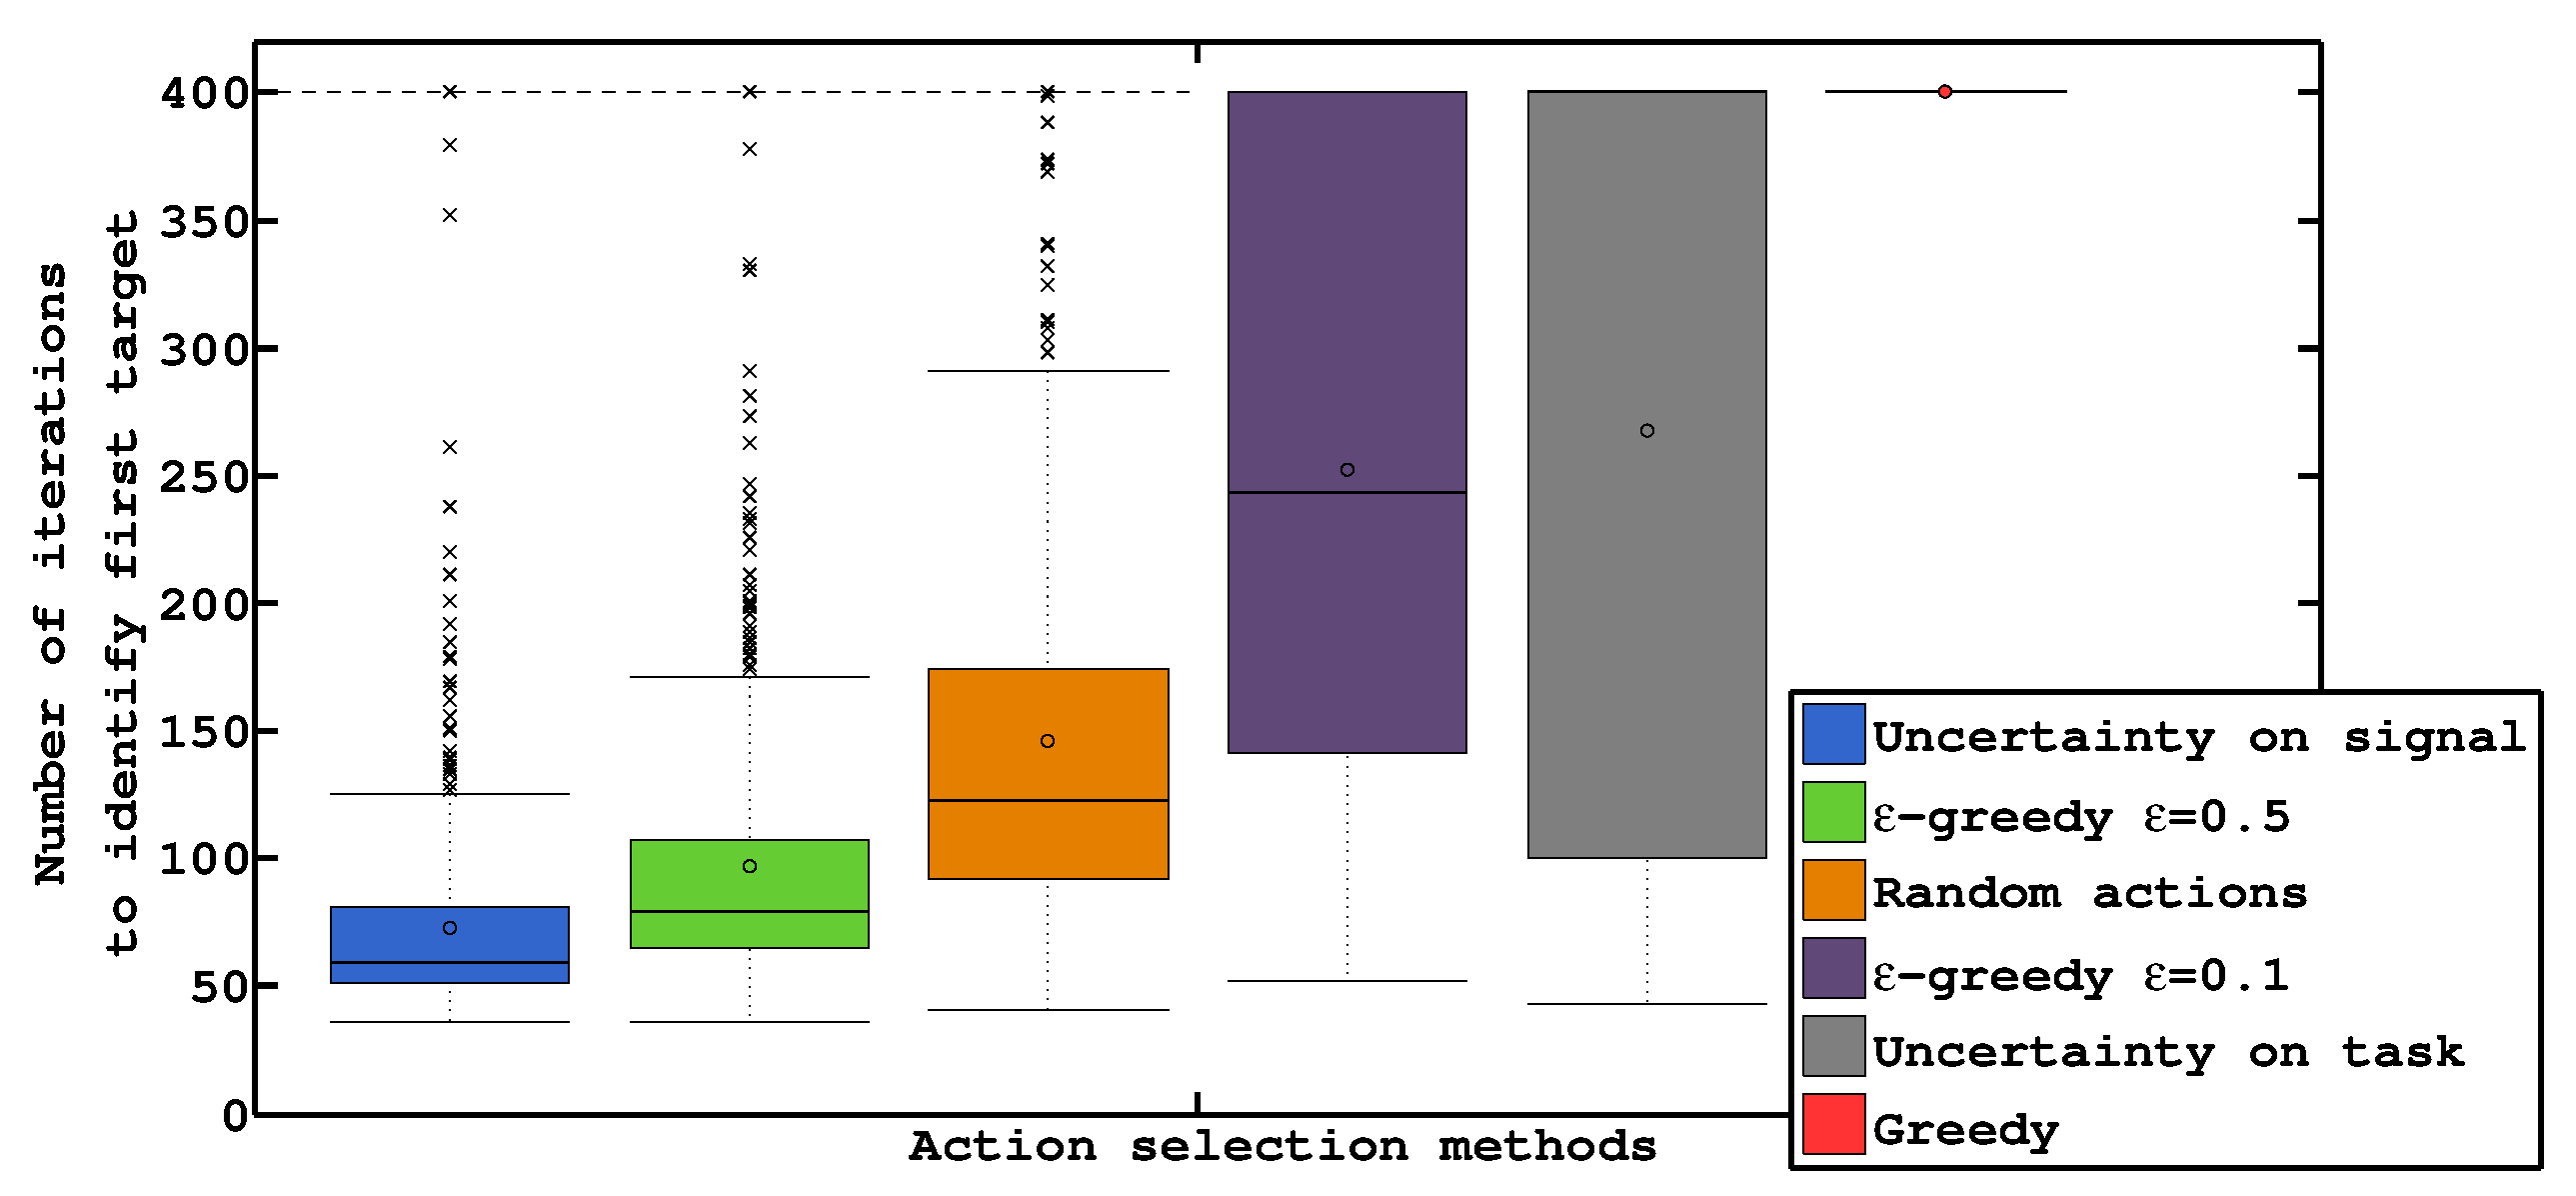
\includegraphics[width=\columnwidth]{\imgpath/battacharyya/plot_planning_first.eps}
    \caption{Comparison of different exploration methods. Our proposed method, based on the uncertainty on the expected signal, allows to lead the system to regions that improve disambiguation among hypotheses in a faster way. For the greedy method, all values were 400 which indicates it never allowed to identify any task.}
    \label{fig:overlapcompplan}
\end{figure}

Figure~\ref{fig:overlapcompplan} shows the results averaged across subjects, runs and datasets. Values of 400 means the confidence threshold was not reached after 400 iterations. Our proposed method, based on the uncertainty on the expected signal, allows to lead the system to regions that improve disambiguation among hypotheses in a faster way. Trying to follow the most probable task does not allow the system to explore sufficiently (Greedy), and at least some random exploration is necessary to allow a correct identification of the task ($\epsilon$-greedy). Assessing uncertainty only on the task performs poorly as it does not take into account the signal interpretation ambiguity inherent to our problem. The large variability in the results is mainly due to the large variations in classification accuracy across subjects and datasets. Given these results, the remainder of this section will only consider our proposed planning method.

\paragraph{Using the Bhattacharyya coefficient in the long run}

After identifying the first task, and following our approach, we continued running the system and measured how many tasks were identified after 400 steps. Figure~\ref{fig:overlapbhatta} demonstrates the advantage of switching to a classification based method after identification of a first target instead of keeping the estimation given by the Bhattacharyya coefficient. On the one hand, Bhattacharyya coefficient works very well for small amounts of data because it directly compares model parameters. On the other hand, after identifying many task, all models share most of their signal-label pairs and it requires much more data to modify the models and detect overlaps. Therefore using a classifier allows for a faster identification since the classifier makes a much harder decision for each new EEG signal. This discussion is in line with the observation on the use of the power information made in chapter~\ref{chapter:bci:priorpower}.

\begin{figure}[!ht]
    \centering
        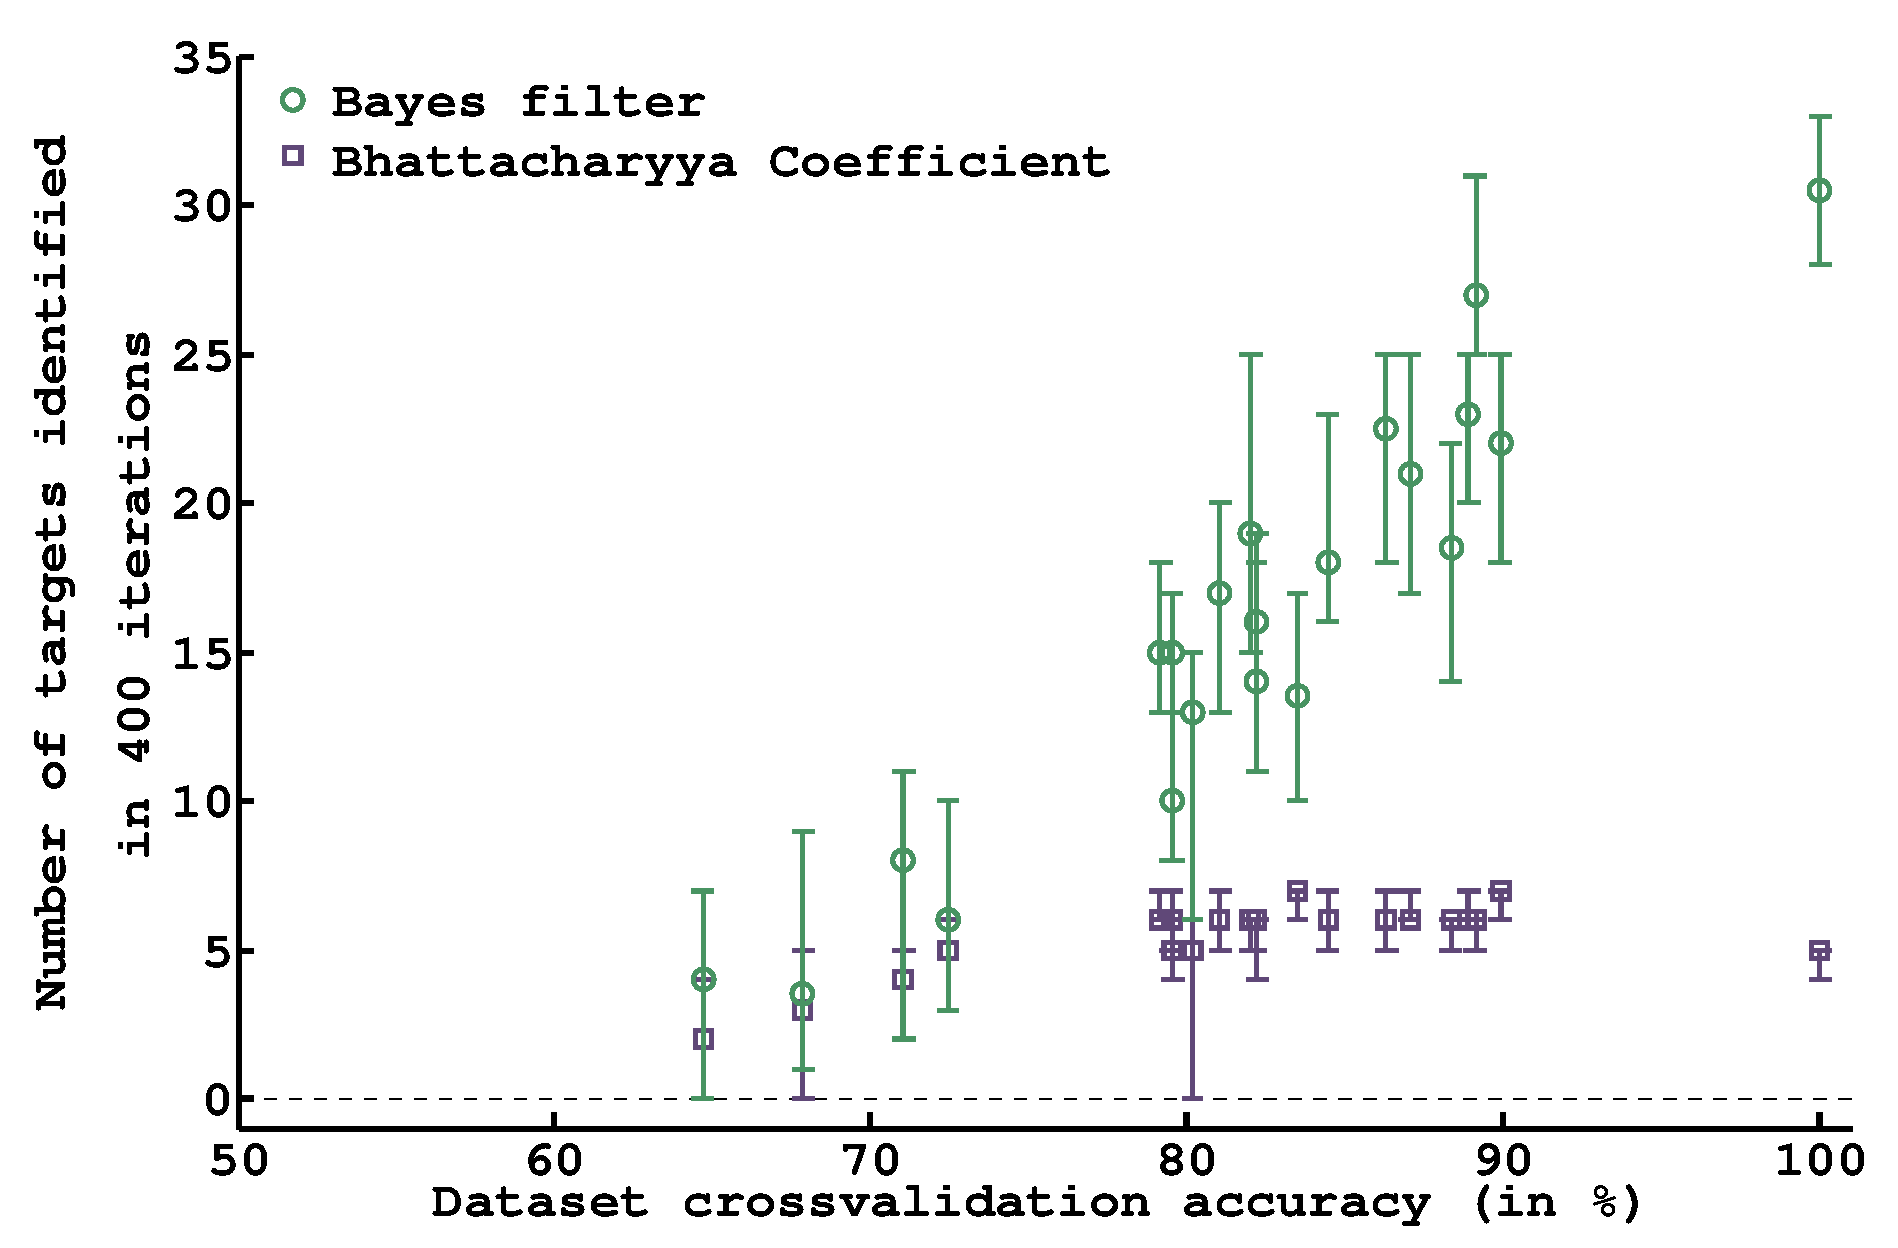
\includegraphics[width=\plotsize\columnwidth]{\imgpath/battacharyya/plot_bhattha_vs_bayes}
        \caption{Number of targets correctly identified in 400 iterations (the markers show the median values and the error bars the 2.5th and 97.5th percentiles). Comparison between switching to a Bayes filter method after identification of a first target instead of keeping the estimation given by the Bhattacharyya coefficient. The classification based method allows for a faster identification.}
        \label{fig:overlapbhatta}
\end{figure} 

Given these results, in the remaining of this section we only consider switching to a classification based method once the first task has been identified.

\paragraph{After 400 steps}

Figure~\ref{fig:overlapavg_sum_400} shows the number of tasks correctly and incorrectly identified in 400 iterations. For datasets of good qualities, we are able to identify more than 20 tasks in 400 iterations without the need for a calibration procedure (recap that previous works needed between 300 and 600 examples for the calibration phase \cite{chavarriaga2010learning,iturrate2010single}). The number of correctly identified tasks is strongly correlated to the quality of the dataset.

\begin{figure}[!ht]
    \centering
    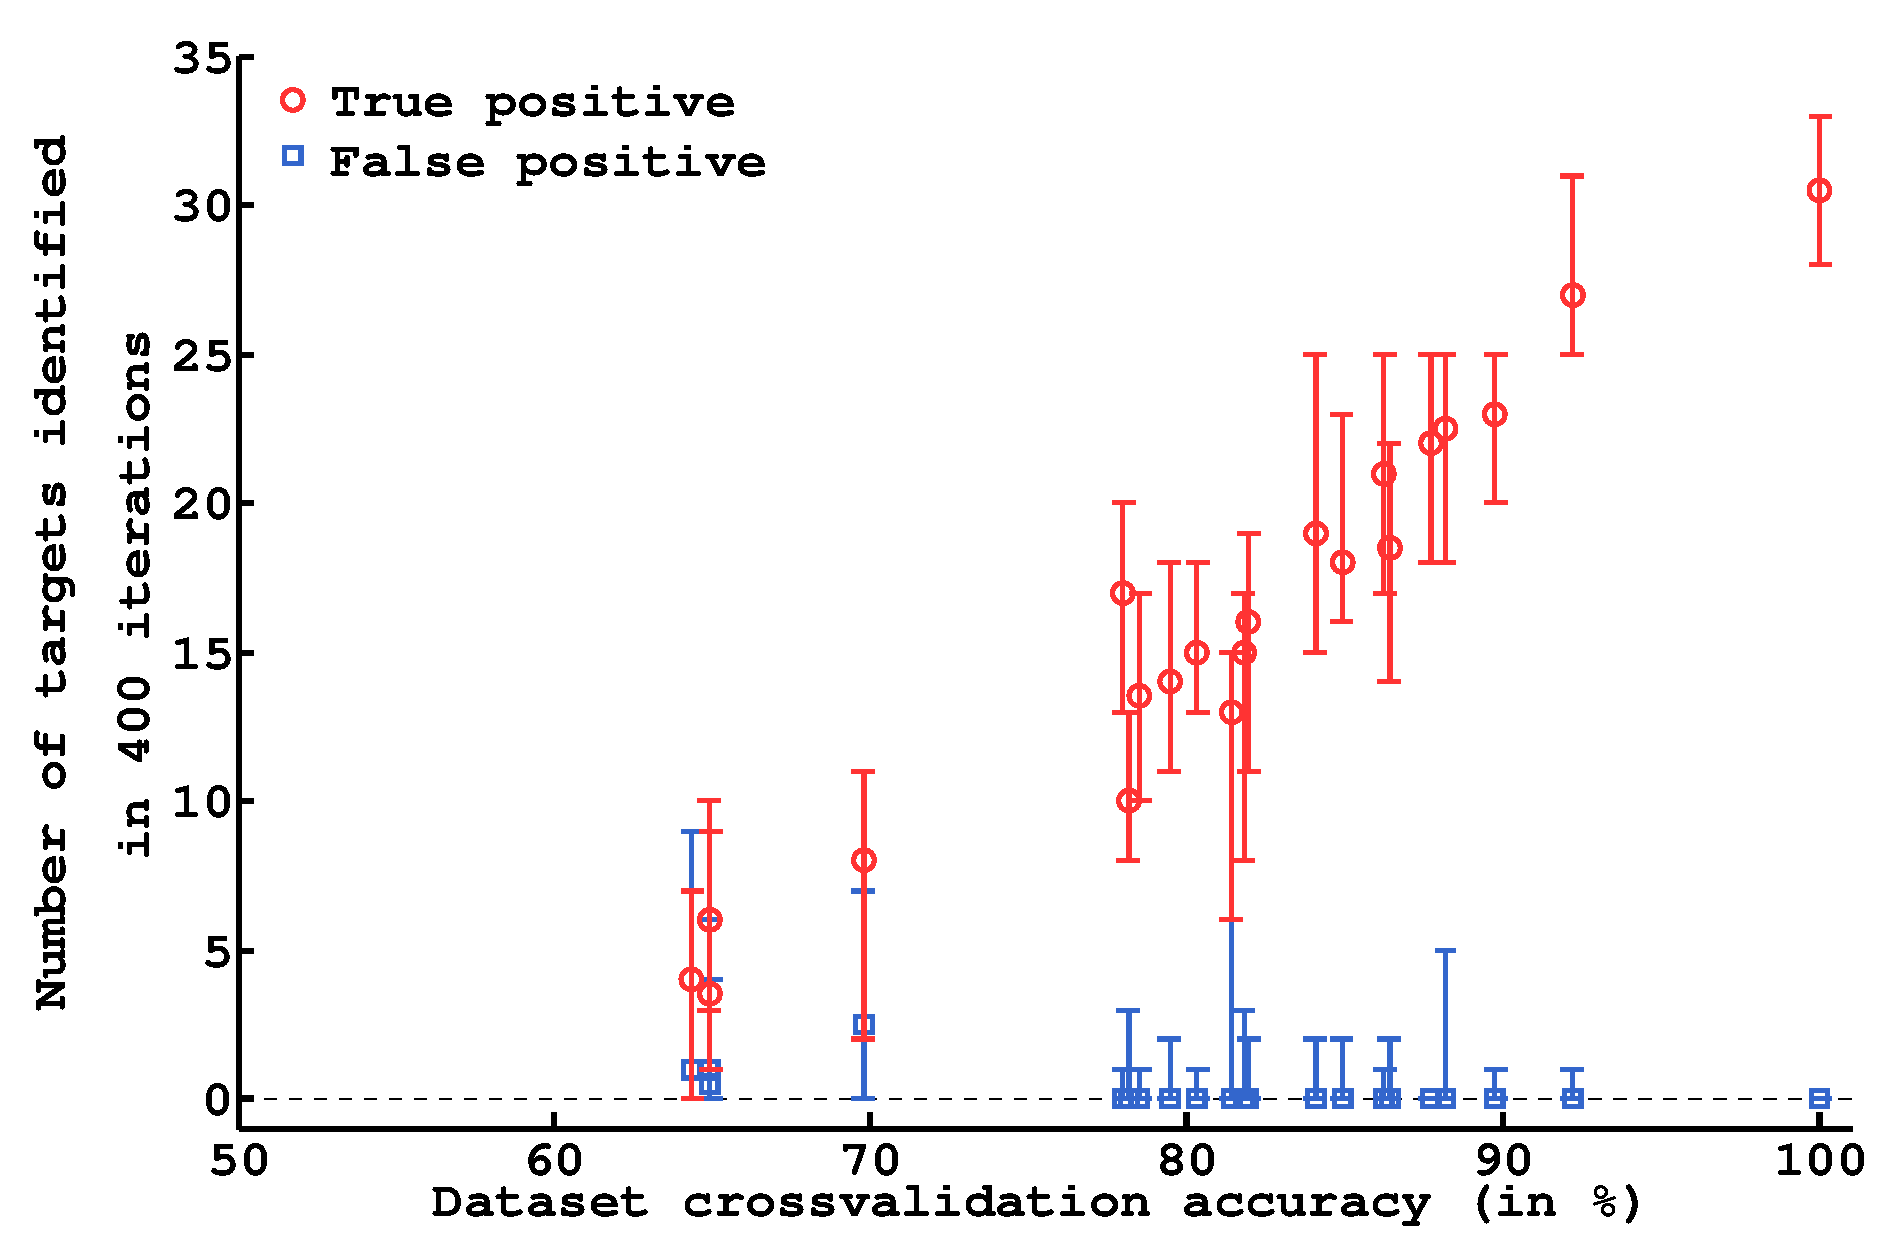
\includegraphics[width=\plotsize\columnwidth]{\imgpath/battacharyya/plot_first400_reach} 
    \caption{Number of targets correctly and incorrectly identified in 400 iterations (the markers show the median values and the error bars the 2.5th and 97.5th percentiles). For datasets of good qualities, we are able to identify more than 20 tasks in 400 iterations without the need for a calibration procedure.}
    \label{fig:overlapavg_sum_400}
\end{figure} 

The quality of our unsupervised method can be measured according to the percentage of labels correctly assigned (according to the ground truth label), see Figure~\ref{fig:overlappercentageLabels}. In general, having dataset with classification accuracies higher than 75$\%$ guaranteed that more than 90$\%$ of the labels were correctly assigned. This result shows that our algorithm can also be used to collect training data for calibrating any other state-of-the-art error-related potentials classifier, but has the important advantage of controlling the device at the same time.

\begin{figure}[!ht]
    \centering
        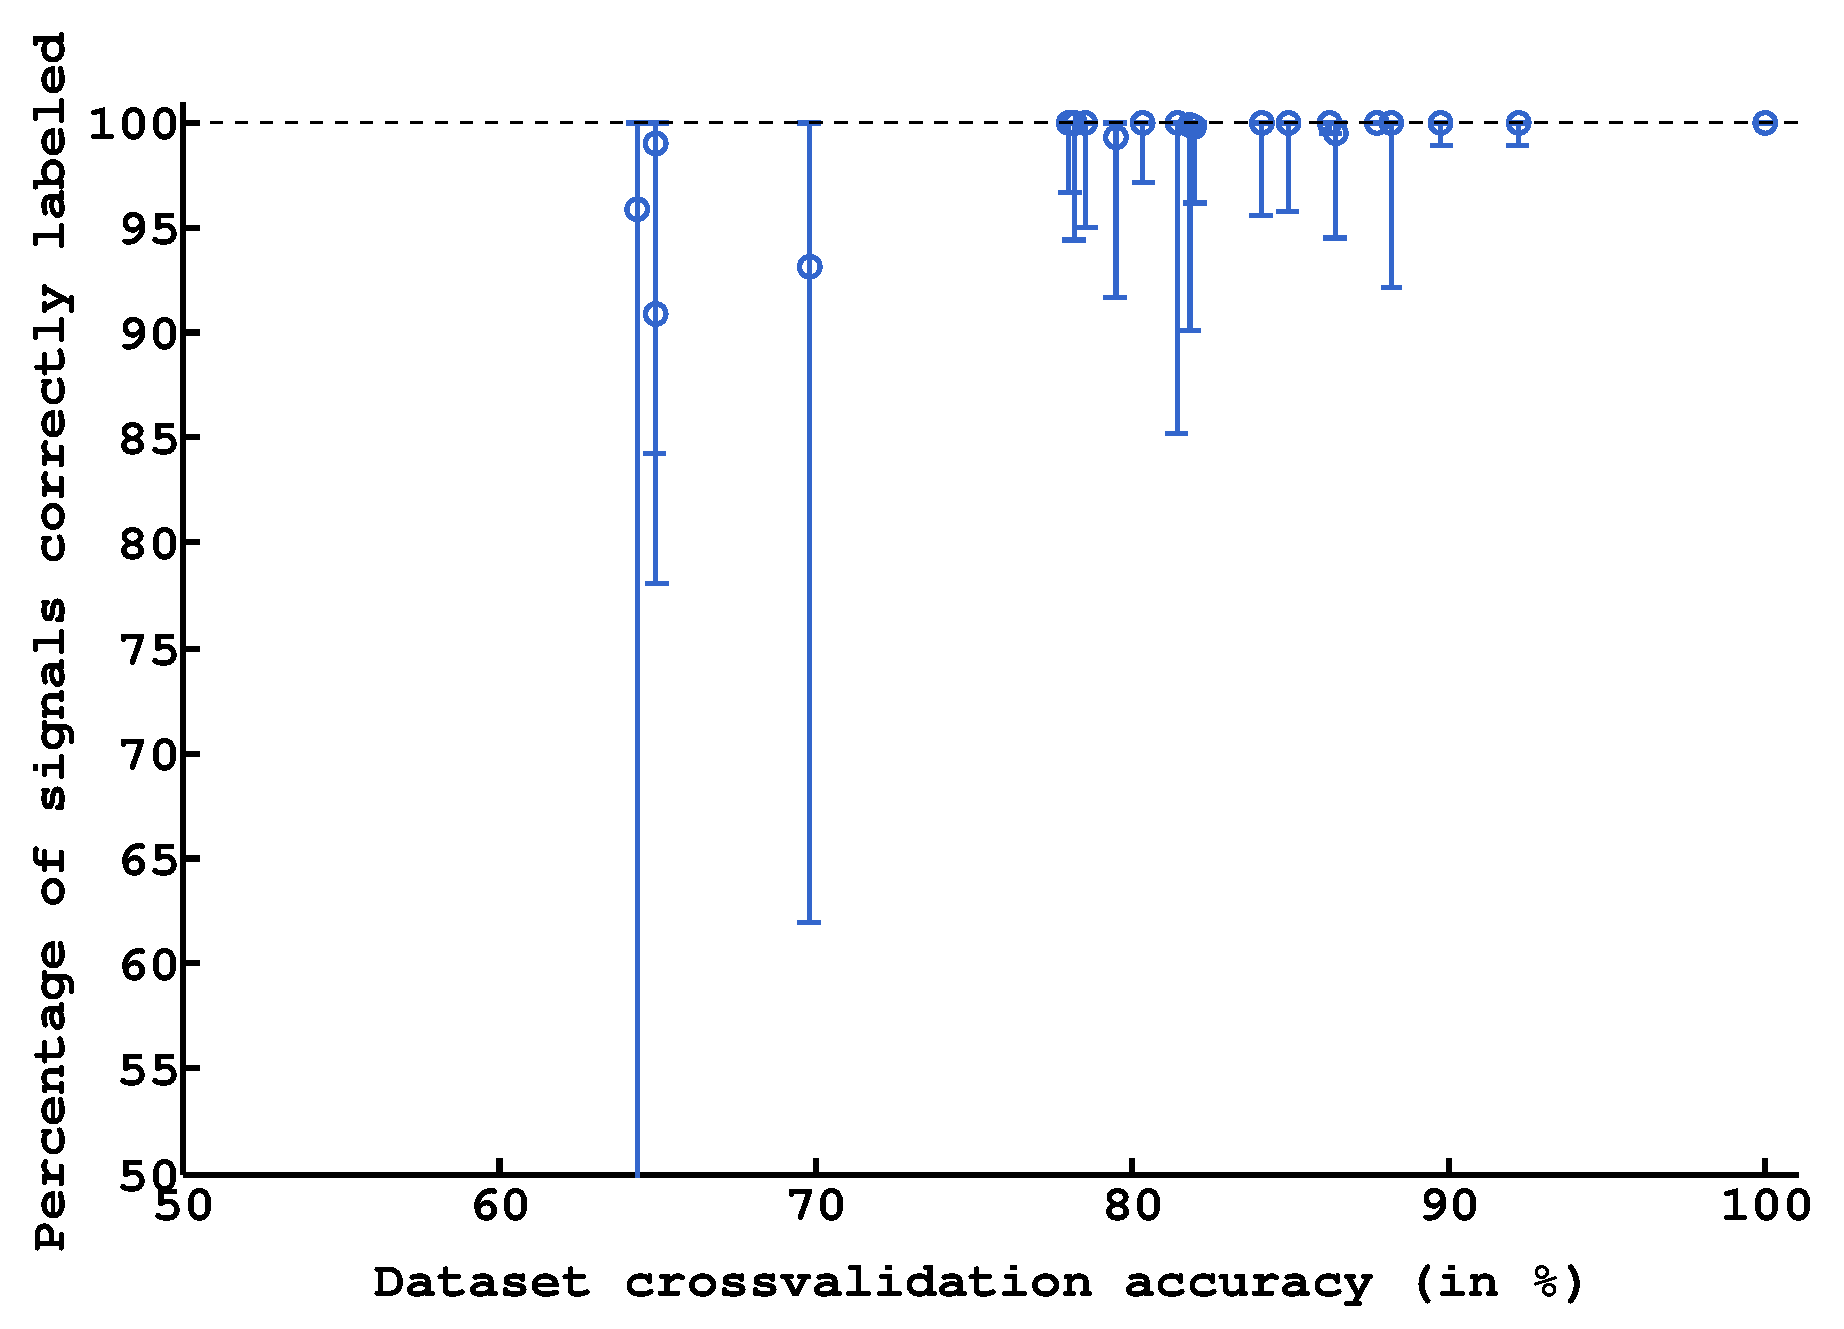
\includegraphics[width=\plotsize\columnwidth]{\imgpath/battacharyya/plot_percent_label}
        \caption{Percentage of labels correctly assigned according to the ground truth label (the markers show the median values and the error bars the 2.5th and 97.5th percentiles). In general, having dataset with classification accuracies higher than 75$\%$ guaranteed that more than 90$\%$ of the labels were correctly assigned.}
        \label{fig:overlappercentageLabels}
\end{figure}

\subsection{Online control}

The experiments were conducted with four subjects (aged between 25 and 28). Each subject was asked to mentally assess the agent's actions with respect to a given target. The system was not calibrated to decode the user EEG signals beforehand. Each subject performed 5 runs, for each run a new target was randomly selected and provided to the user. There was an action every three seconds. Each run lasted 200 actions, and the time between runs was around one minute.

The algorithm was able to identify the correct target for all runs of all the subjects, see Figure~\ref{fig:overlaponlineresults}. There are strong variations among subjects but we note that our system identified each task in less iterations than a normal calibration phase requires (between 300 and 600 examples depending on the user performance \cite{chavarriaga2010learning,iturrate2010single}).

\begin{figure}[!ht]
    \centering
    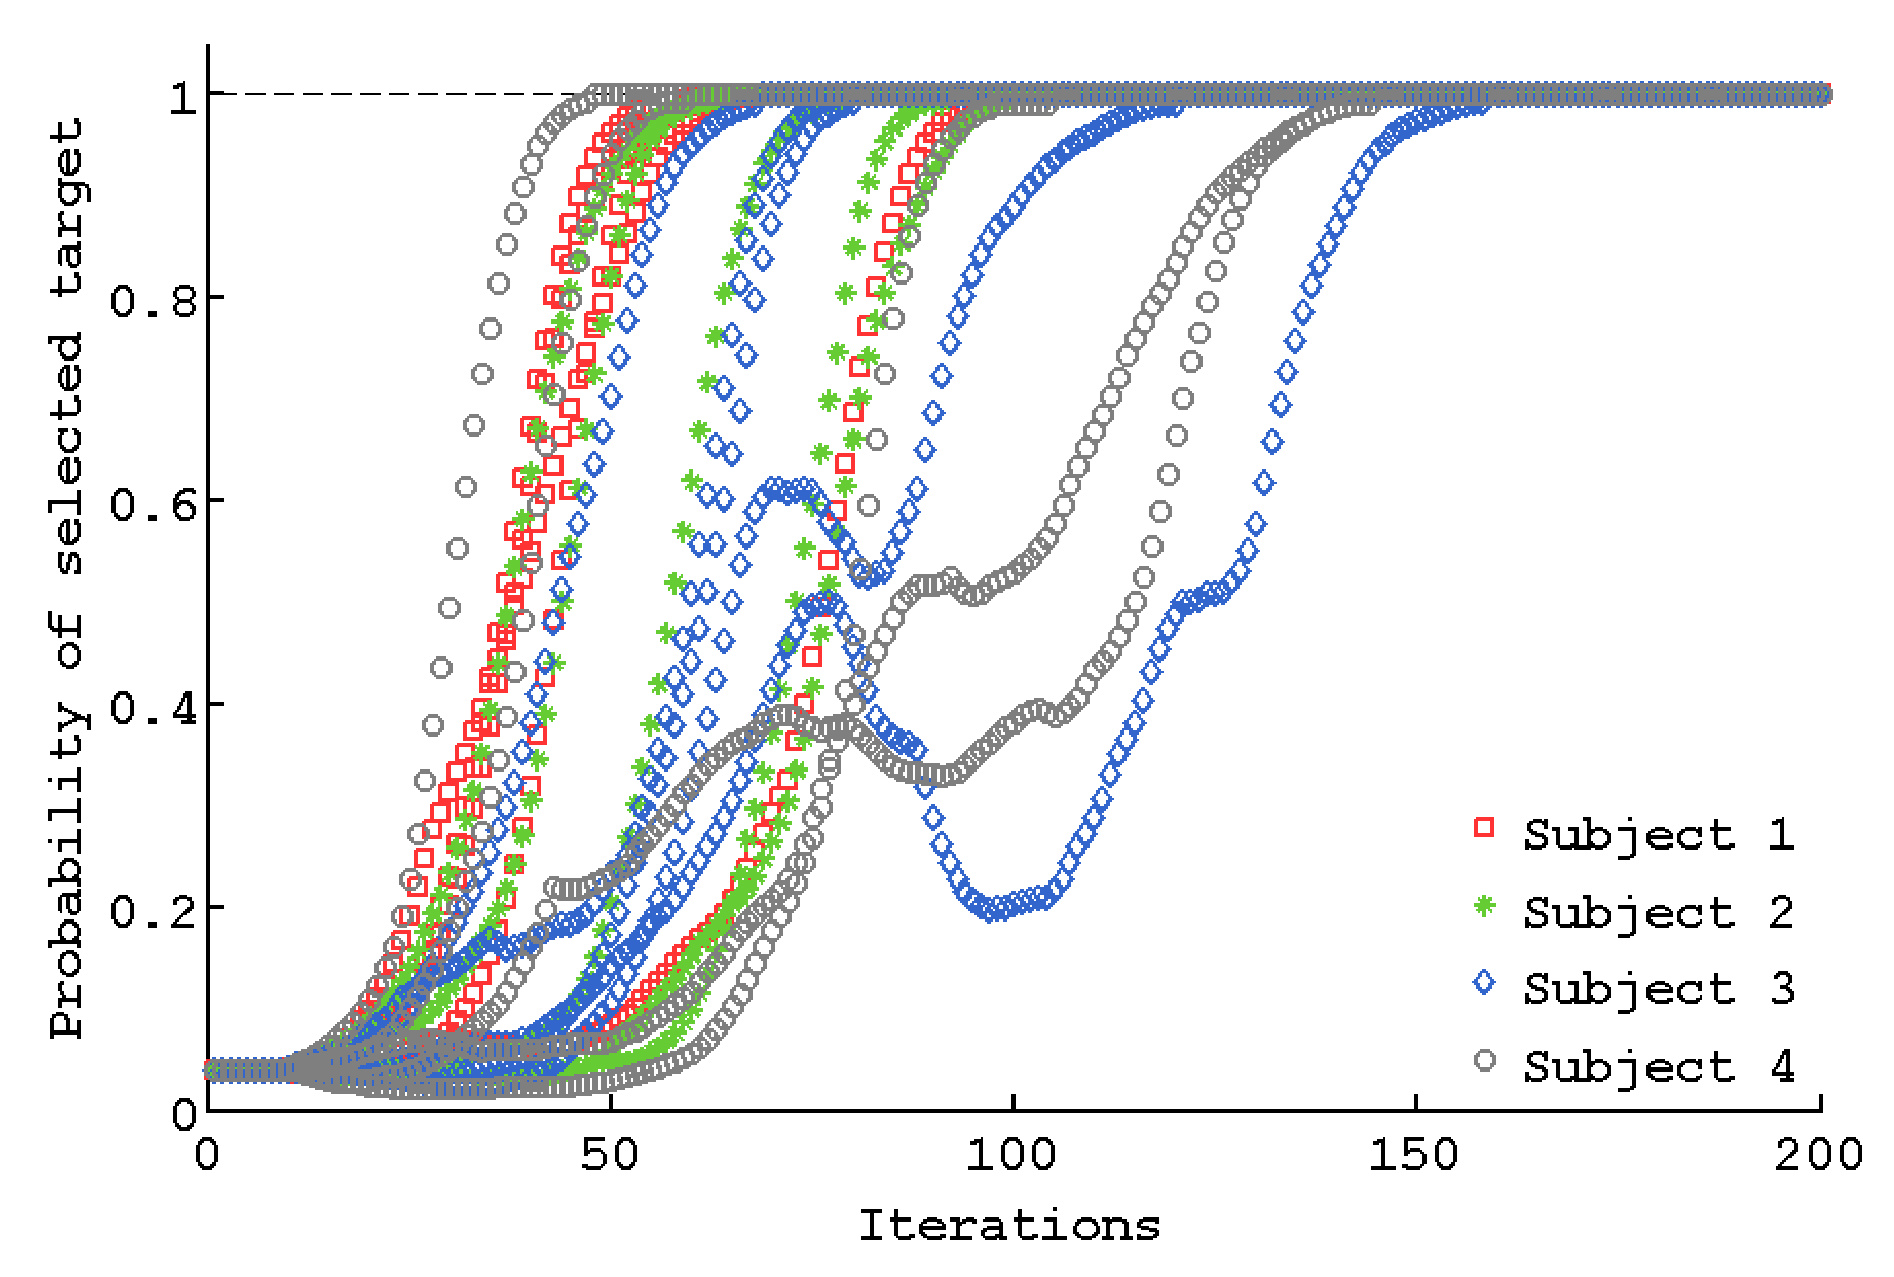
\includegraphics[width=\plotsize\columnwidth]{\imgpath/battacharyya/plot_realevolution}    
    \caption{Results from the online experiments: Evolution of the probability of the correct task for each subject and run. The algorithm was able to identify the correct target for each subjects and runs in less than 200 iterations.}
    \label{fig:overlaponlineresults} 
\end{figure}

Table~\ref{tab:overlaponline} shows for each subject and run the number of iterations needed to reach the confidence threshold for the subject selected target.

On average, the number of iterations needed to identify the target was of 85 $\pm$ 32.

\begin{table}[!ht]
\centering
\rowcolors{2}{gray!25}{white}
\begin{footnotesize}
\begin{tabular}{r|rrrrr|r}
    %\toprule
    & \textbf{Run1} & \textbf{Run2} & \textbf{Run3} & \textbf{Run4} & \textbf{Run5} & \textbf{mean$\pm$std} \\\hline
    %\midrule
    \textbf{S1} & 95 & 62 & 56 & 60 & 64 & 67 $\pm$ 16 \\
    \textbf{S2} & 89 & 77 & 98 & 60 & 62  & 77 $\pm$ 17 \\
    \textbf{S3} & 68 & 80 & 118 & 76 & 157 & 100 $\pm$ 37 \\
    \textbf{S4} & 98 & 142 & 57 & 142 & 47 & 97 $\pm$ 45 \\
\end{tabular}
\end{footnotesize}
  \caption{Results from the online experiments: Number of iterations needed to identify the correct target for each subject and run. On average, the number of iterations needed to identify the target was of 85 $\pm$ 32.}
  \label{tab:overlaponline}
\end{table}

\subsection{Discussion}

We introduced a new method to exploit the facts that, when associated hypothetic labels to all task hypothesis, only the correct task assign the correct labels to the correct hypothesis. This method compares directly the overlap between the distribution modeling the generation of such signals. As for wrong hypothesis, the labels tend to be mixed with respect to the underlying structure of the data, the overlap between distribution is a good and stable measure. 

However, we have seen that once all hypothesis share the same signal-label pairs, this method requires to collect more and more data to detect a change in the overlap of the wrong hypothesis. As a consequence the system should make use of two different sets of equations, one specific to the first target and one for the forthcoming targets.

This latter aspect shows the important advantage of the method we presented in this thesis, which only make use of one equation from the first to the last iteration. This equation captures both phase of the interaction, where during a first phase the classifier qualities are playing a major role, and in a second phase the classifier predictions are taking the lead by taking more hard decisions.

%%%%%%%%%%%%%%%%%%%%%%%%%%%%%%%%%%%%%%%%%%%%%%
%%%%%%%%%%%%%%%%%%%%%%%%%%%%%%%%%%%%%%%%%%%%%%
%%%%%%%%%%%%%%%%%%%%%%%%%%%%%%%%%%%%%%%%%%%%%%
%%%%%%%%%%%%%%%%%%%%%%%%%%%%%%%%%%%%%%%%%%%%%%
%%%%%%%%%%%%%%%%%%%%%%%%%%%%%%%%%%%%%%%%%%%%%%
\section{A frame is a generic function}

demo some frame, remind it can include any specific detail known


%%%%%%%%%%%%%%%%%%%%%%%%%%%%%%%%%%%%%%%%%%%%%%
%%%%%%%%%%%%%%%%%%%%%%%%%%%%%%%%%%%%%%%%%%%%%%
%%%%%%%%%%%%%%%%%%%%%%%%%%%%%%%%%%%%%%%%%%%%%%
%%%%%%%%%%%%%%%%%%%%%%%%%%%%%%%%%%%%%%%%%%%%%%
%%%%%%%%%%%%%%%%%%%%%%%%%%%%%%%%%%%%%%%%%%%%%%
%!TEX root = ../../thesis.tex
\section{Continuous state space}
\label{chapter:limitations:continousstate}

\question{How to deal with continuous states?}

As for now, our algorithm assumes the world can be represented by a limited number of discrete states. In this section we extend our algorithm to a continuous world, but still consider discrete actions. In addition, we present a new interaction frame that combines the feedback and guidance frames. We investigate how our algorithm scales to such problem and how different exploration strategies perform.

\subsection{Experimental System}

We consider a puddle world, in which an agent must reach a goal region while avoiding a penalty region. We consider a 2 dimensional puddle world with each dimension ranging between 0 and 1. The state of the agent can be any coordinate in the 2D world. Agent' actions are discrete and represent steps in either North, South, East, West direction. One step length is sampled from a normal distribution of mean 0.1 and standard deviation 0.01.

As in the experiment of chapter~\ref{chapter:lfui}, we consider speech as the modality for interacting with the robot and we reuse the dataset presented in section~\ref{chapter:lfui:speechdata}. The interaction between the agent and the teacher follows a turn taking social behavior, where the agent is performing an action and waits for a feedback or guidance signal to continue. We only consider a Gaussian classifier.

\paragraph{Task Representation} 

To define the set of possible tasks we project a 5x5 regular grid on top of the continuous world. One task is represented by a +1 reward in one of the 25 projected squares and a -100 reward in three consecutive (vertically or horizontally) squares. +1 and -100 area can not overlap (see figure~\ref{fig:puddle} for an example). The set of possible tasks is defined as all possible combinations of such reward function, for a total of 660 hypotheses.

Our algorithm only needs to have access to the optimal policies to be able to interpret a signal with respect to the feedback or guidance frame. We use the MDP framework to compute the corresponding policies. The world being continuous we use the tile coding function approximation \cite{sutton1998reinforcement}, with 10 overlapping 50x50 regular grids. A Q-Learning algorithm \cite{watkins1992q} is used to compute the Q-Values, with a discount rate of 0.99 and a learning rate of 0.01. The optimal policies are then defined as greedy according to the Q-Values.

\paragraph{Mixed feedback and guidance frame}

In previous chapters, we considered only the feedback or the guidance frame separately. Such limitation can be restrictive for the user, we  now consider the case where the teacher can use both feedback and guidance signal. We define as $F$ as the set of meanings associated to the feedback meanings (i.e. ``correct'' and ``incorrect''), and $G$ the set of meanings associated to the guidances meanings (i.e. ``action 1'', ``action 2'', ...). Extending our algorithm to cases where possible meanings include both feedback and guidance (i.e. $l^f \in \{F \cup G\}$) requires a probabilistic model of how the teacher distributes feedback and guidance signals. This model must hold the following property $\sum_{l \in \{F \cup G\}} p(l^f = l|s,a,\xi)~=~1$. We define a variable $\phi$ that represents the probability of the user providing a feedback signal at each step, i.e. $p(l^f \in F) = \phi$, which implies $p(l^f \in G) = 1 - \phi$.

Under this new definition we can change our frame definition to:

\begin{eqnarray}
    p(l^f = l|s,a,\xi) = 
        \begin{cases} 
            \phi~p(l^f = l|s,a,\xi) &\mbox{for } l \in F \\
            (1- \phi)~p(l^f = l|s,\xi) & \mbox{for } l \in G
        \end{cases}
        \label{eq:mixedfeedbackguidance}
\end{eqnarray}
where Equation~\ref{eq:feedbackframe} holds for the feedback component (for $l \in F$) and Equation~\ref{eq:guidanceframe} holds for the guidance component (for $l \in G$). 

We assume the mixing parameter $\phi$ is known in advance. We set $\phi$ to 0.5 meaning the user is providing feedback half of the time and guidance the other half of the time. 

\paragraph{Exploration strategies}

We investigate four different agent behaviors: \begin{inparaenum}[a)] \item random, \item $\epsilon$-greedy, \item myopic uncertainty based exploration, which aims at selecting the action that is the most uncertain in the current state, and \item full uncertainty based exploration which requires an uncertainty map to decide what to explore next. \end{inparaenum} 

As we are in a continuous domain, we can not compute the full uncertainty for each state as presented in chapter~\ref{chapter:planning}, we therefore approximate this process. Extensions of the general problem already exist for the continuous state problem \cite{nouri2010dimension,Hester13aamas} and we will rely on a sampling based method. One hundred random states are generated and evaluated in terms of their uncertainty. Each sampled state is associated to a reward value proportional to its uncertainty which is propagated to neighborhood states by using a fixed Gaussian kernel. We use as amplitude the uncertainty value and a diagonal covariance matrix of value 0.01 for each component. The resulting approximated uncertainty map is then used as a reward function. By solving the corresponding MDP, using for instance Q-Learning, the agent plans its actions to visit the most uncertain regions. We decided to use an $\epsilon$-greedy policy on the Q-values. In the following experiment, the agent will use an exploration ratio $\epsilon$ equal to $0.1$.

\subsection{Results}

We present results from 75 runs of our experiment, where for each run we randomly choose a task to teach from the set of hypotheses, as well as the initial state of the agent. The simulated teacher makes 10 percent of teaching mistakes, i.e. sending an erroneous signal 10 percent of the time. For each experiment, we compute the likelihoods every 15 steps and performs a total of 35 updates, for a total of 525 iterations. Figure~\ref{fig:continuousstateRmax} shows the average evolution of the taught task hypothesis likelihood.

\begin{figure}[!htbp]
  \centering
  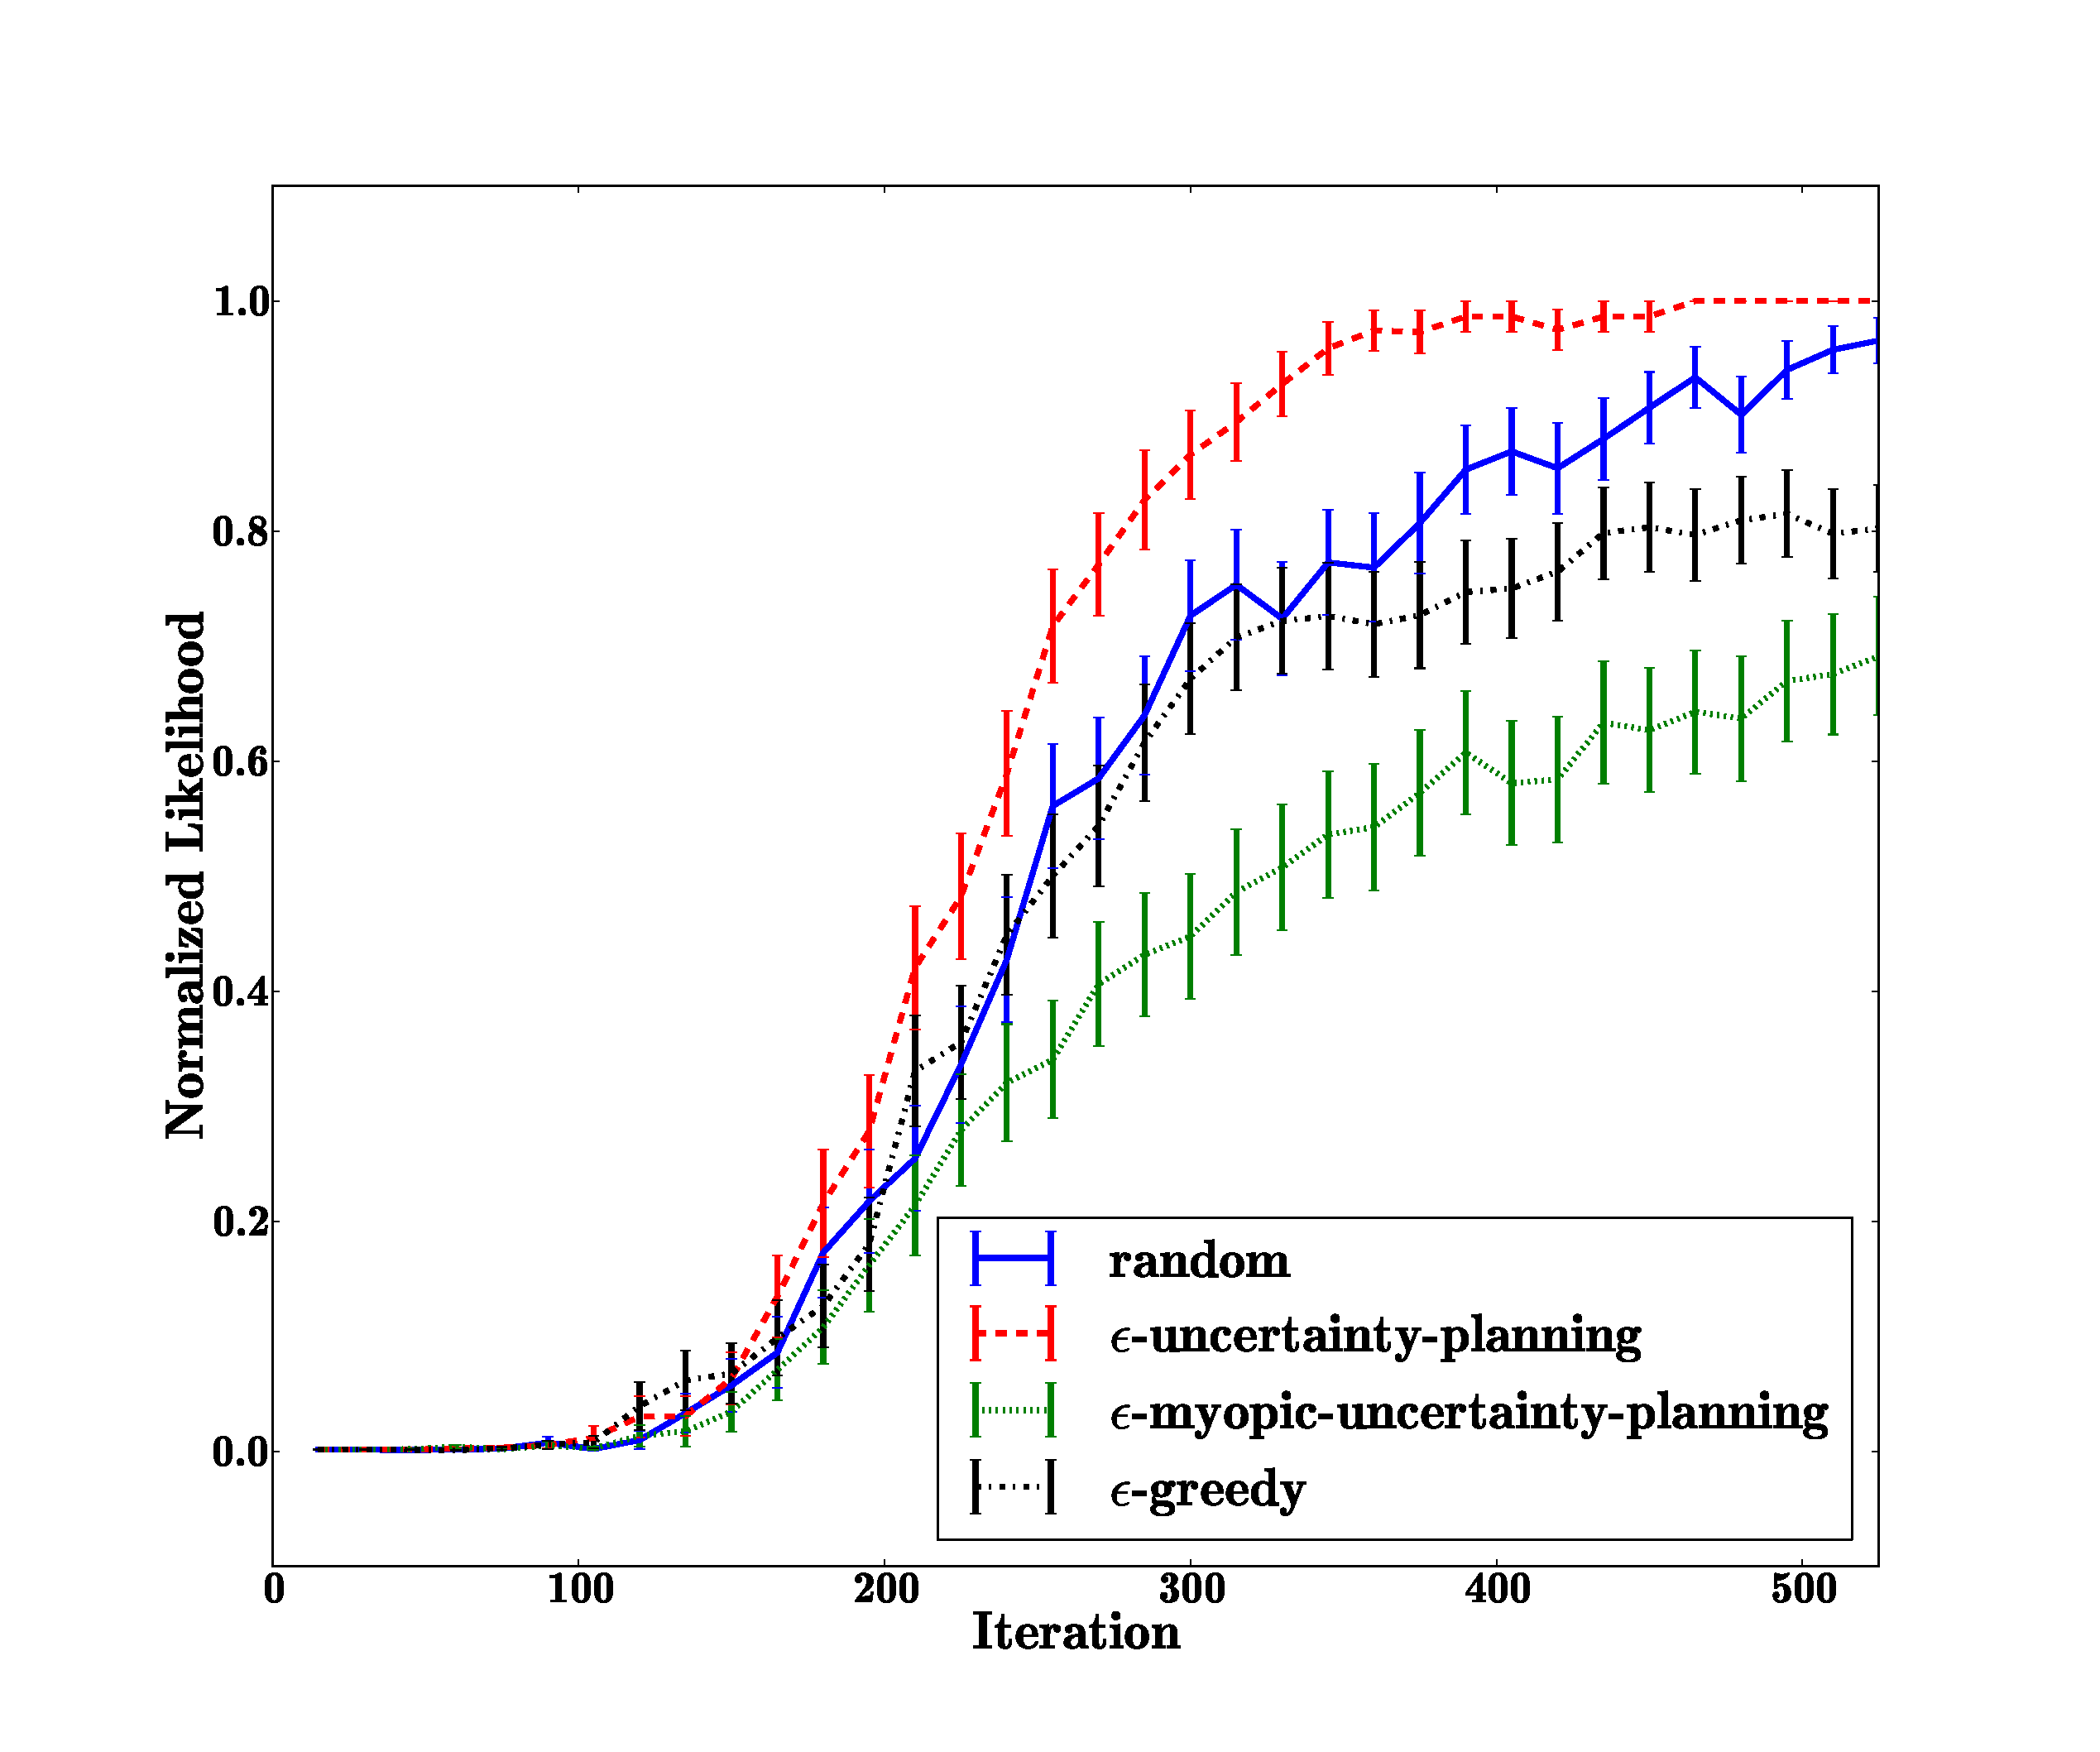
\includegraphics[width=\plotsize\columnwidth]{\imgpath/continuous_state/continuous}
  \caption{Taught hypothesis normalized likelihood evolution (mean + standard error) thought iteration using a Gaussian classifier. Comparison of different exploration strategies. Uncertainty based exploration method, which plan on the long term, performs significantly better on average.}
  \label{fig:continuousstateRmax}
\end{figure}

These results show that our algorithm can learn a task in a continuous world from unlabeled and noisy instructions whose possible meanings are both feedback and guidance and 10 percent of the instructions were teaching mistakes. The uncertainty based planning strategy outperforms random action selection. Interestingly, myopic uncertainty based strategy, which is also based on our uncertainty measure, is not efficient. This result illustrates that, when considering the agent as not being able to teleport, a long term planning approach is more suited to explore efficiently the state space than a short term vision by selecting the next action with higher immediate reward, i.e. higher uncertainty. 

% Finally $\epsilon$-greedy performs less efficiently than in the first setup. This is due to the properties of our new set of hypothesis where many hypothesis shared an identical positive reward area but have different puddle zone.

Figure~\ref{fig:continuousstateUncertaintyMap} shows the evolution of the estimated uncertainty map for one run of the experiment. For each uncertainty map, the agent plans its actions to reach a maximal uncertainty region. The maximum uncertainty value decreases as the agent is correctly estimating the task.

\begin{figure}[!htbp]
  \centering
      \begin{subfigure}[b]{0.35\columnwidth}
          \centering
          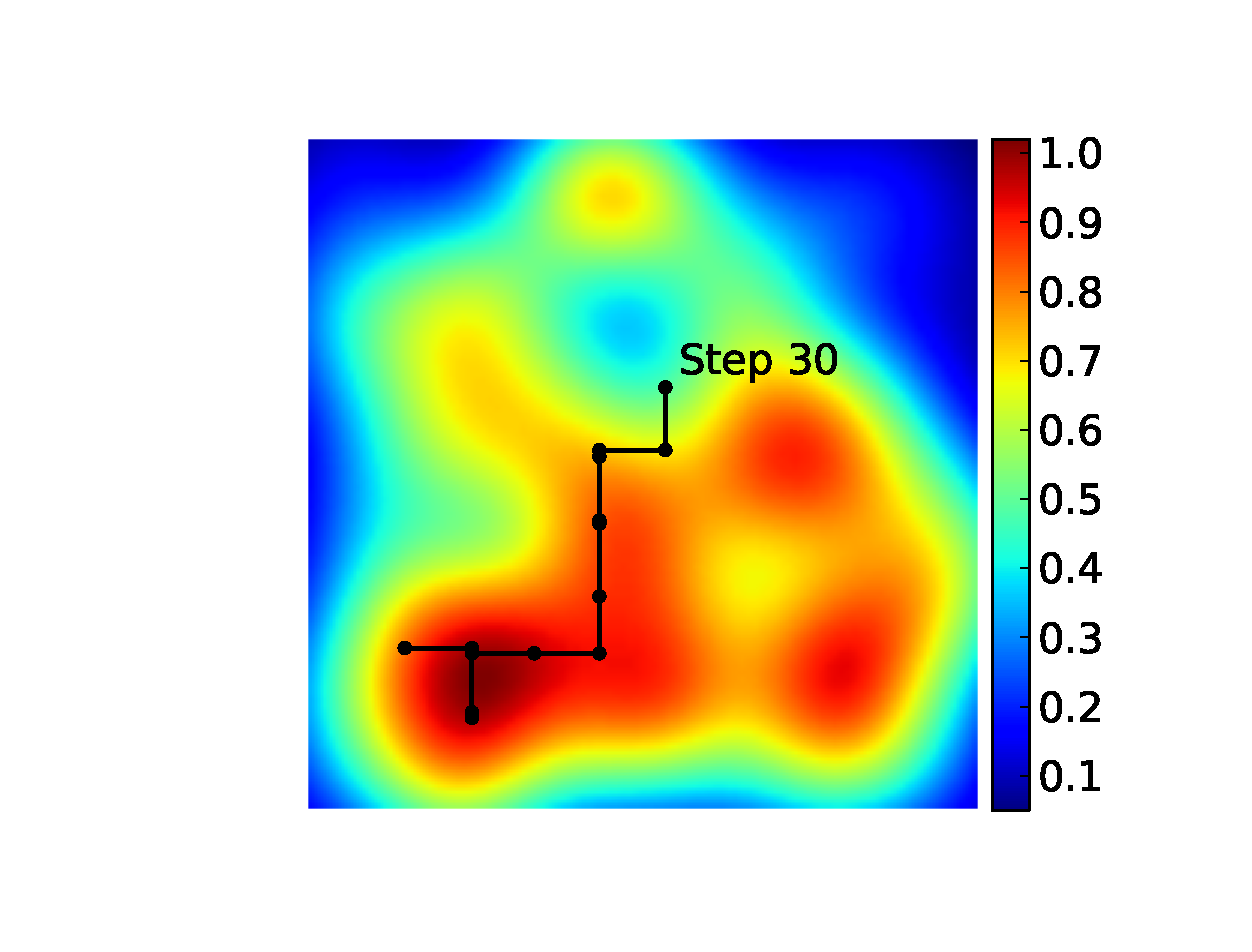
\includegraphics[trim=5cm 1.5cm 1.5cm 1.5cm, clip=true, width=\columnwidth]{\imgpath/continuous_state/30}
          \caption{After 30 iterations.}
          \label{fig:30}
      \end{subfigure}
      \begin{subfigure}[b]{0.35\columnwidth}
          \centering
          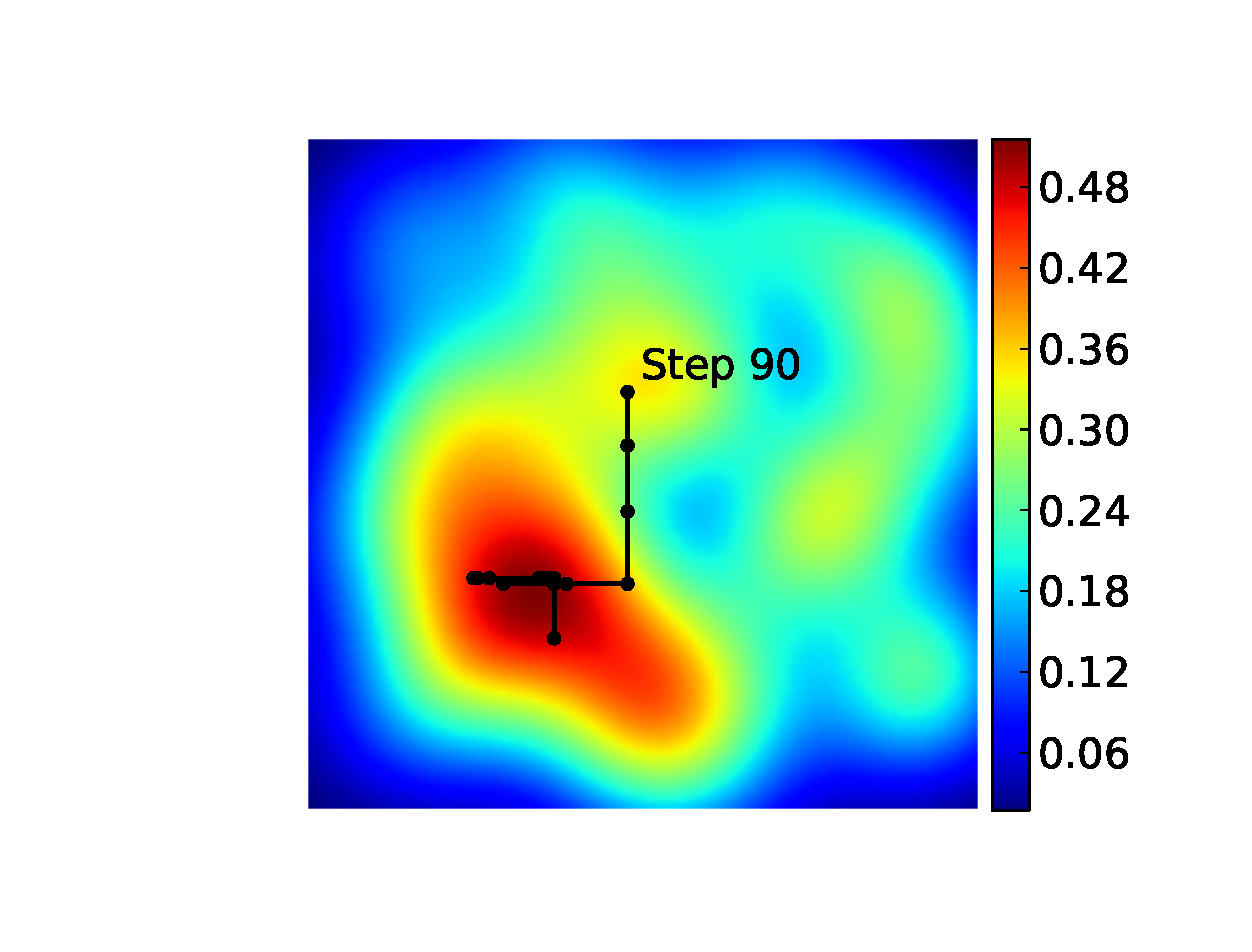
\includegraphics[trim=5cm 1.5cm 1.5cm 1.5cm, clip=true, width=\columnwidth]{\imgpath/continuous_state/90}
          \caption{After 90 iterations.}
          \label{fig:90}
      \end{subfigure}\\
      \begin{subfigure}[b]{0.35\columnwidth}
          \centering
          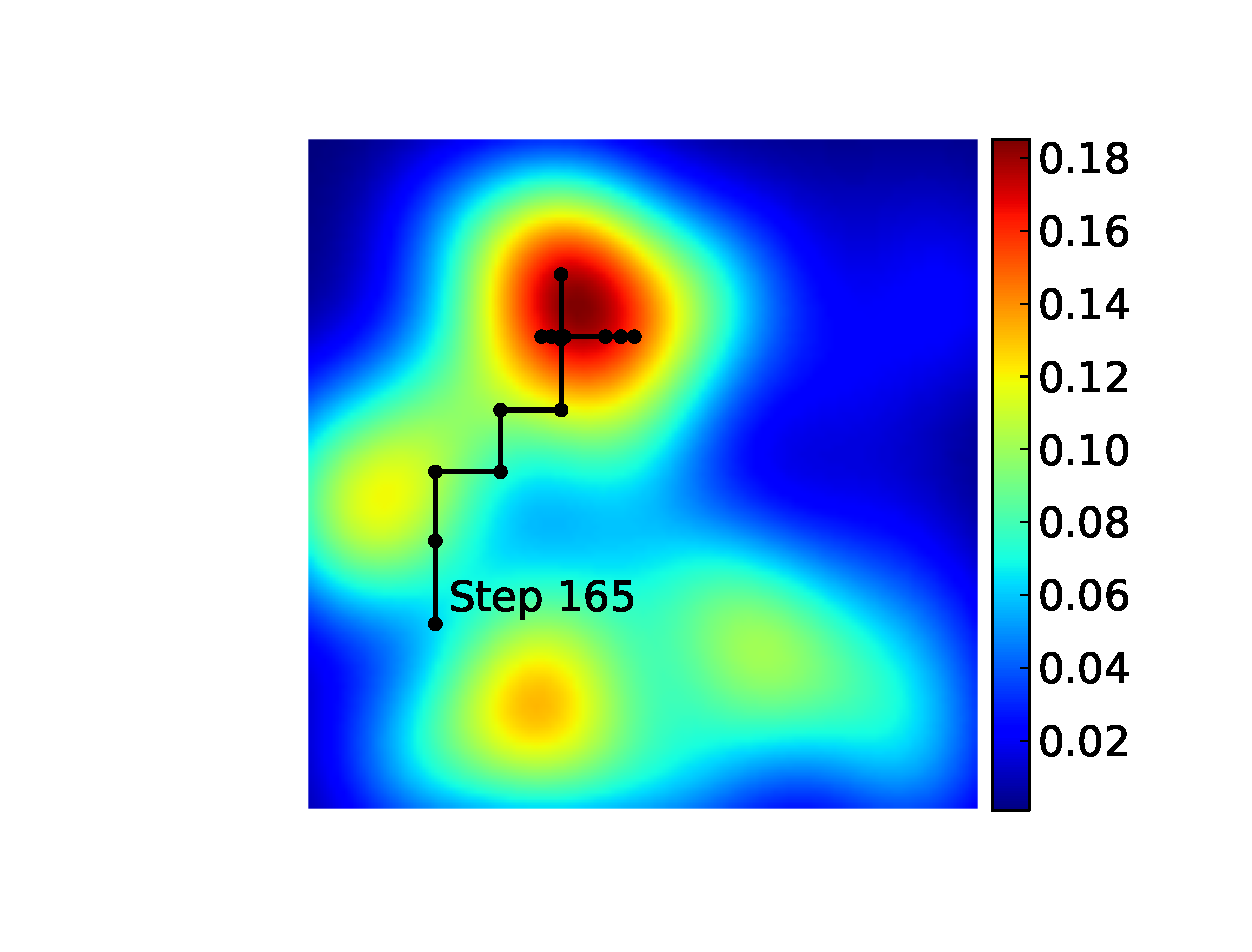
\includegraphics[trim=5cm 1.5cm 1.5cm 1.5cm, clip=true, width=\columnwidth]{\imgpath/continuous_state/160}
          \caption{After 165 iterations.}
          \label{fig:165}
      \end{subfigure}
      \begin{subfigure}[b]{0.35\columnwidth}
          \centering
          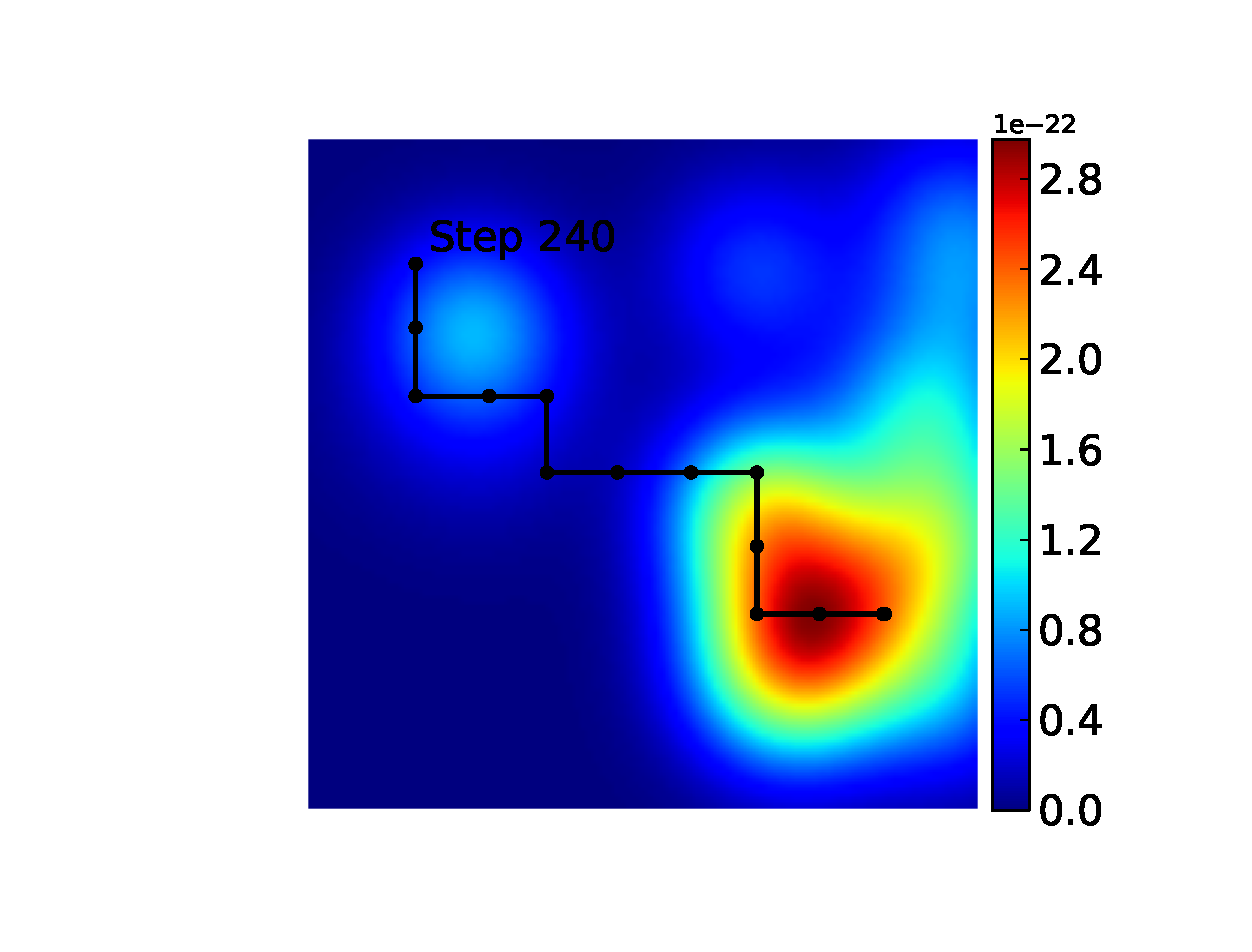
\includegraphics[trim=5cm 1.5cm 1.5cm 1.5cm, clip=true, width=\columnwidth]{\imgpath/continuous_state/240}
          \caption{After 240 iterations.}
          \label{fig:240}
      \end{subfigure}\\
      \begin{subfigure}[b]{0.25\columnwidth}
          \centering
          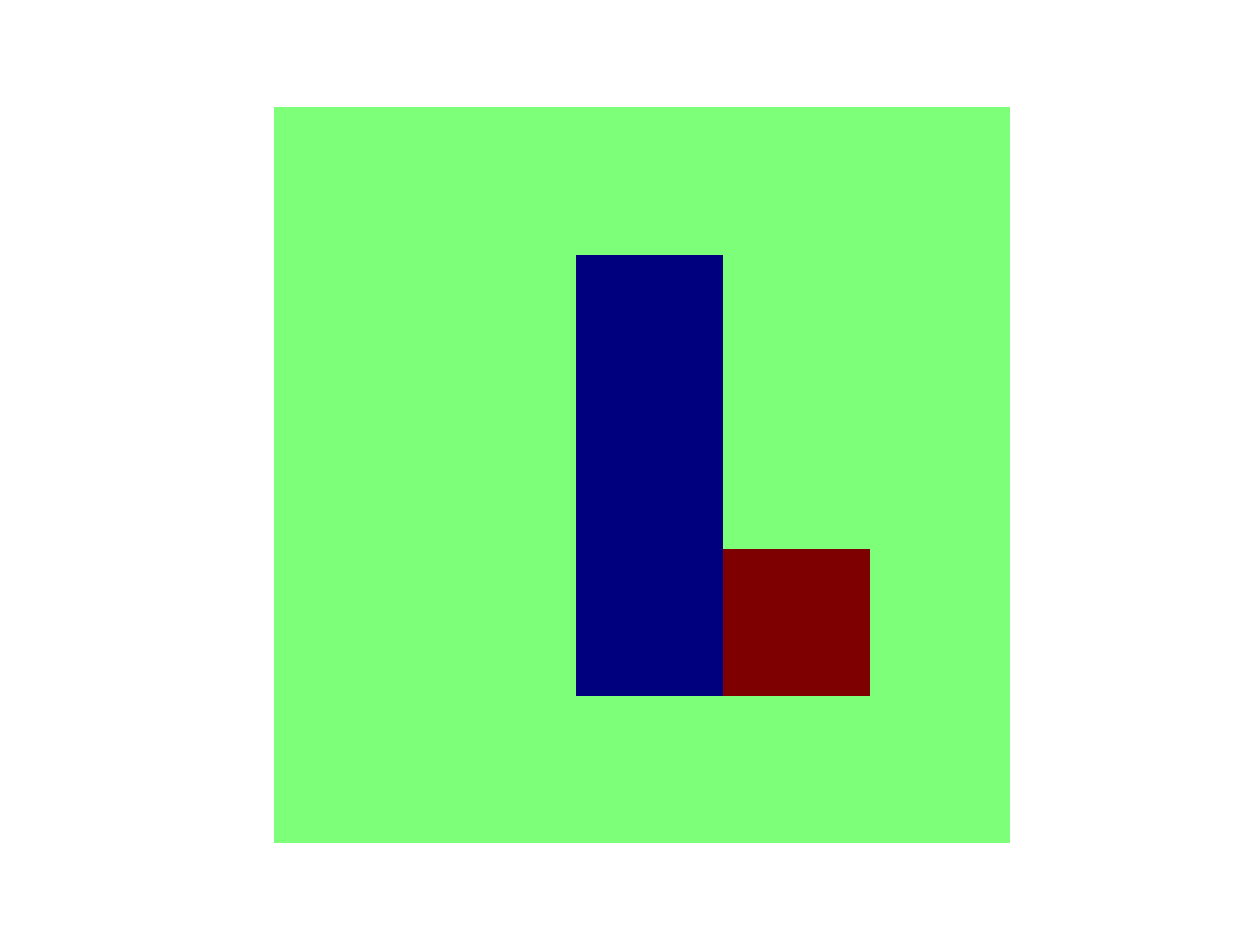
\includegraphics[trim=4cm 1cm 3.5cm 1cm, clip=true, width=\columnwidth]{\imgpath/continuous_state/puddle}     
          \caption{Puddle world used by the teacher.}
          \label{fig:puddle}
      \end{subfigure}
      \begin{subfigure}[t]{0.45\columnwidth}
          \centering
          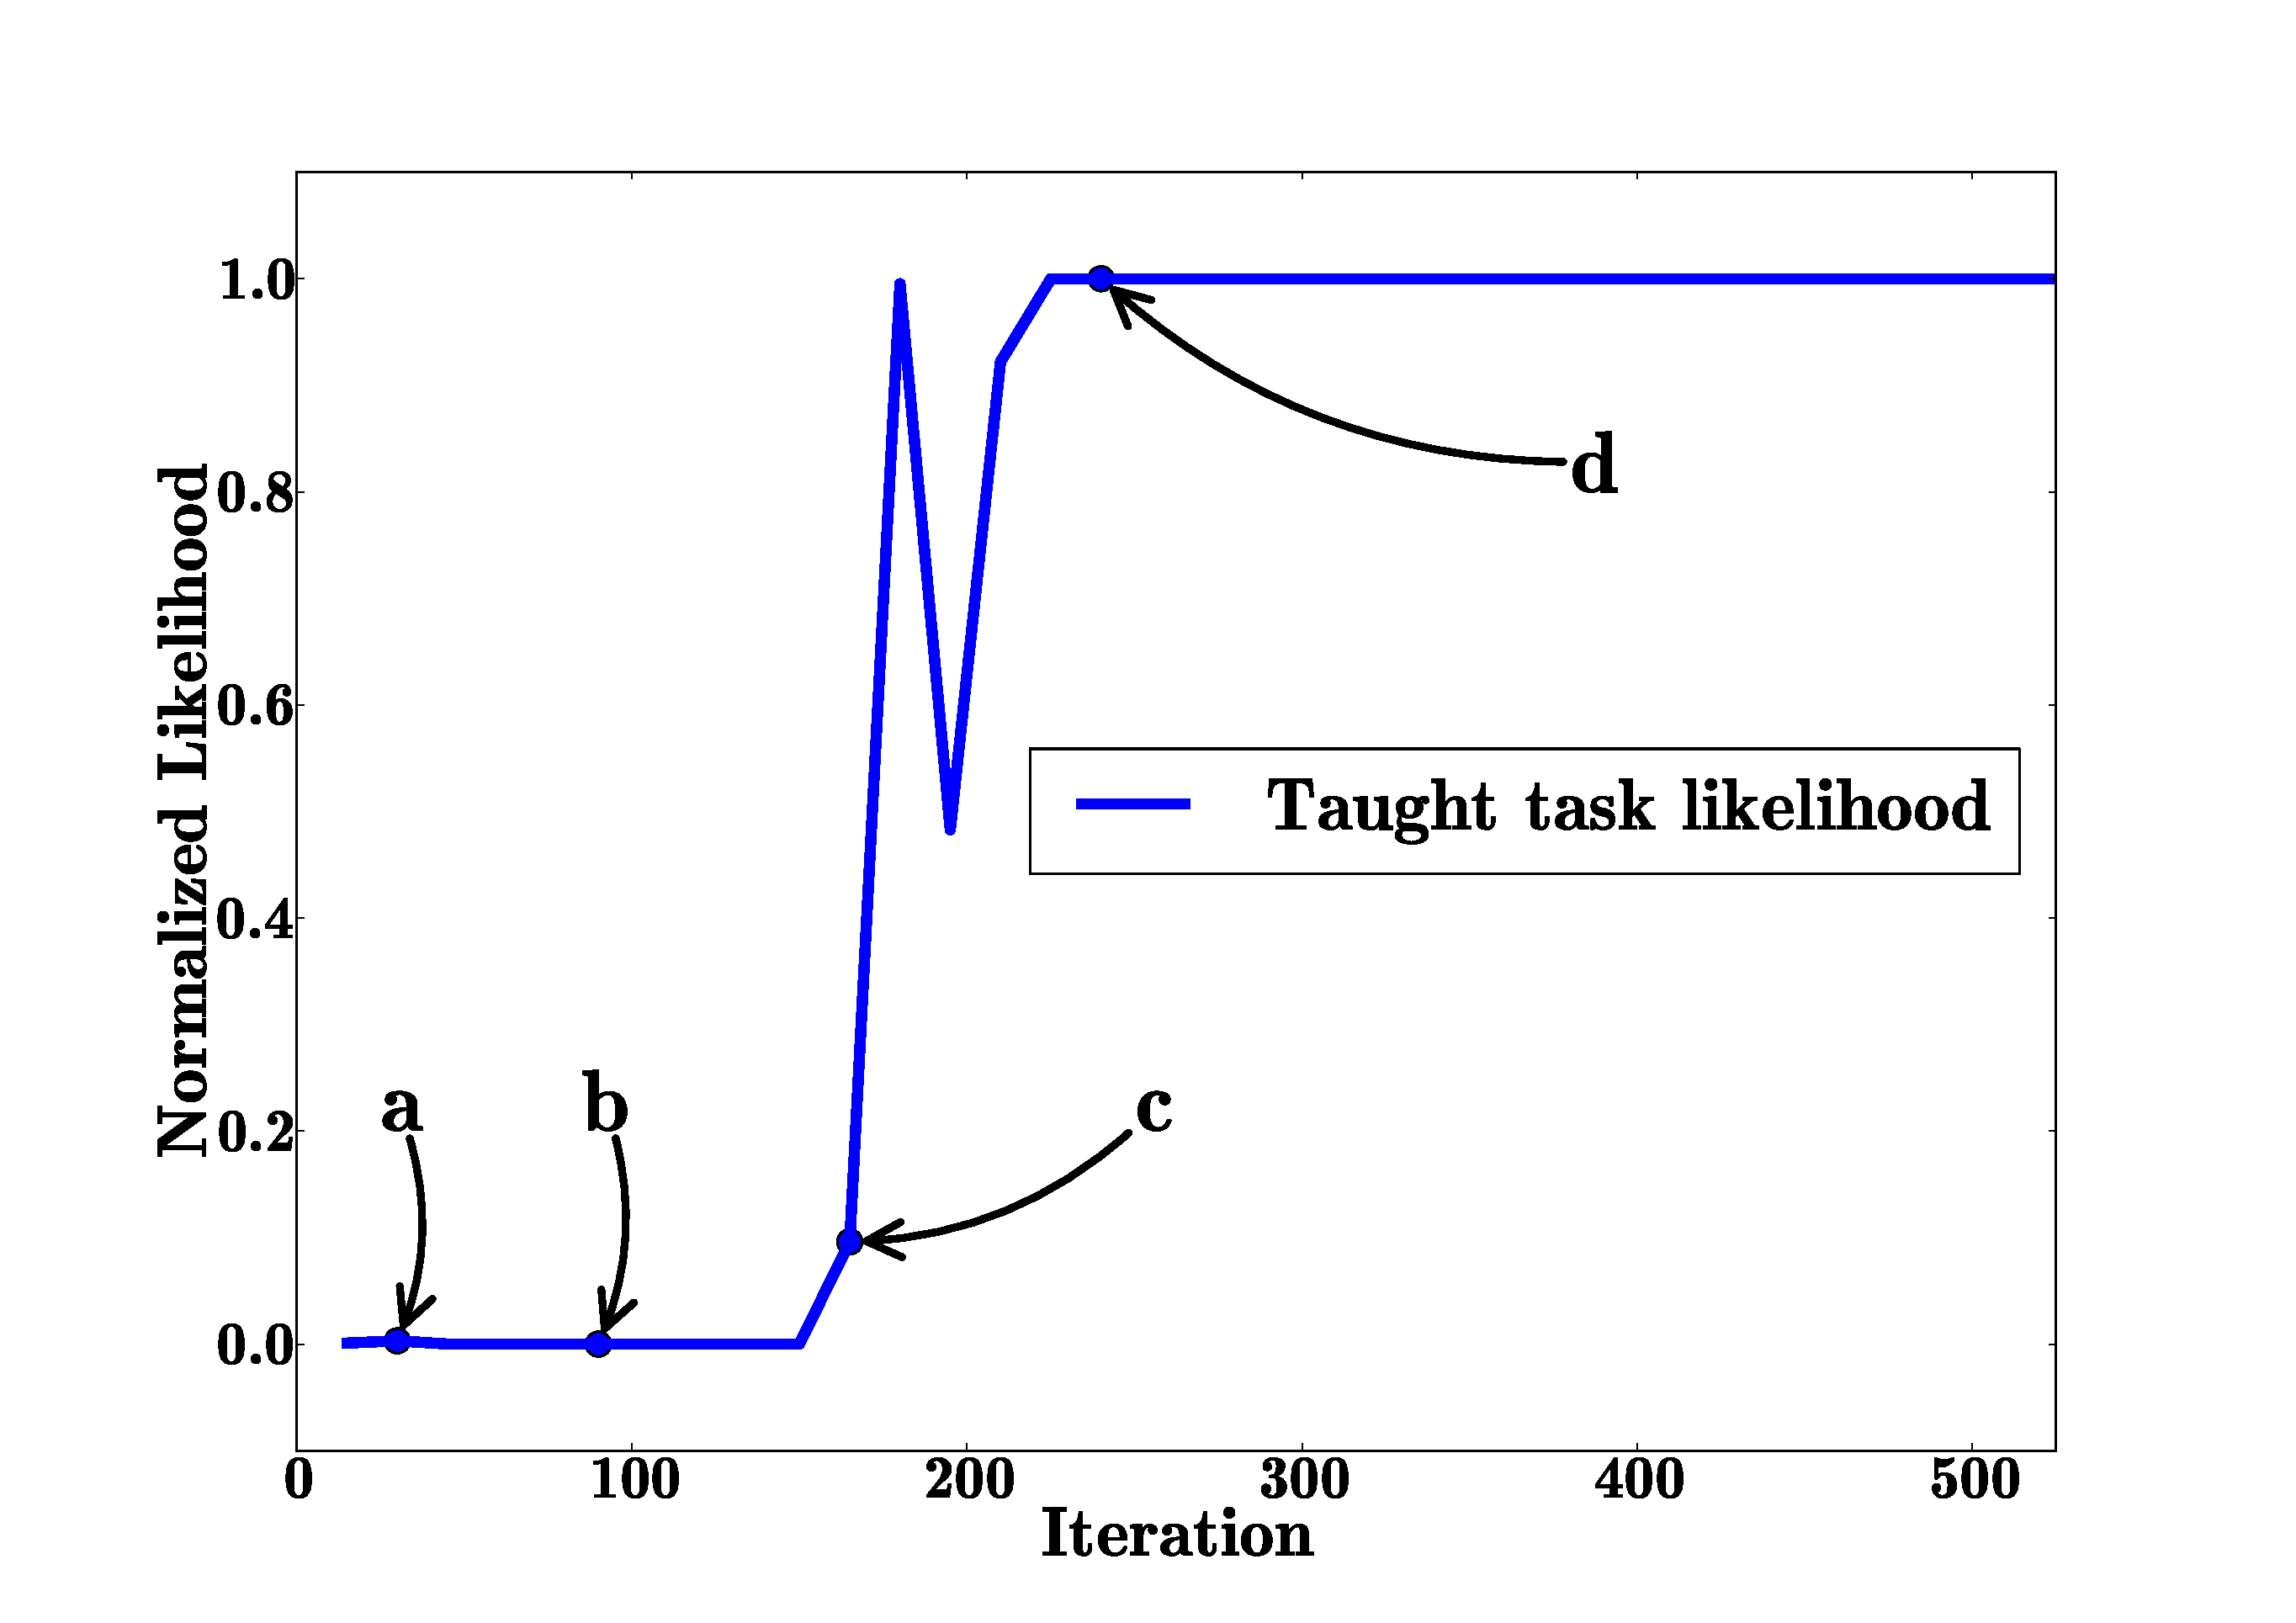
\includegraphics[trim=2cm 1cm 3cm 2cm, clip=true, width=\columnwidth]{\imgpath/continuous_state/evo}
          \caption{Taught hypothesis normalized likelihood evolution.}
          \label{fig:evo}
      \end{subfigure}
        
  \caption{Log Uncertainty maps after a) 30, b) 90, c) 165 and d) 240 iterations. e) shows the puddle world chosen by the teacher and f) shows the learning progress and the frame associated to each of the uncertainty map. In order to display the differences between log values, we bounded the color map between -5 and 0, which correspond to uncertainty values between 0.0067 and 1. Some log values, especially for d), are lower than -5 and are displayed in the same color as -5. Best shown in color.}
  \label{fig:continuousstateUncertaintyMap}
\end{figure}

\subsection{Discussion}

We have shown how our algorithm could be applied to continuous state domains and seen that, given the interaction frame considered, our algorithm only needs to have access to the optimal policies associated to each task to be able to interpret a signal. Therefore any method that allow to compute a policy for continuous domains could be used. The only problem is then related to the computational cost of those methods than to the formalism of this work. We will see in next section that, for some specific frames and worlds, it is not always needed for the robot to know the optimal policies to interpret the teaching signals from the human, which can considerably reduce the computational cost of running our algorithm.


%%%%%%%%%%%%%%%%%%%%%%%%%%%%%%%%%%%%%%%%%%%%%%
%%%%%%%%%%%%%%%%%%%%%%%%%%%%%%%%%%%%%%%%%%%%%%
%%%%%%%%%%%%%%%%%%%%%%%%%%%%%%%%%%%%%%%%%%%%%%
%%%%%%%%%%%%%%%%%%%%%%%%%%%%%%%%%%%%%%%%%%%%%%
%%%%%%%%%%%%%%%%%%%%%%%%%%%%%%%%%%%%%%%%%%%%%%
%!TEX root = ../../thesis.tex

\section{Continuous set of hypothesis}
\label{chapter:limitations:continoushypothesis}

\question{How to leverage from the finite set of hypothesis constraint?}


In order to make the learning problem tractable, it was assumed that the robot learner knows that the task to be learnt can be approximated by one task among a pre-defined set of tasks. Indeed, without constraining the space of possible tasks, an infinite number of task may explain the particular teaching data received by the robot. In practice, the number of pre-defined tasks in the experiment was still relatively large, allowing a certain level of flexibility. Yet, it would be highly desirable to extend the possibility to deal with continuous task representation, allowing potentially infinite spaces of tasks. 

A potential avenue to address this is to constrain search through a combination of regularization and particle filter approaches. In the following of this section, we present a simple particle filter based algorithm that allow an agent to identify a task from unlabeled instruction and considering an infinite set of hypothesis. The agent evolve in a 2 dimensional continuous state and should identify which one of the infinite amount of possible state it should reach.

\subsection{World and task}

We consider an agent living in a 2 dimensional continuous space bounded between 0 and 1 in both dimension. A teacher is providing indication about the orientation of the goal state compared to the robot state by drawing some patterns on a tablet. Those direction can only be selected among of the four cardinal directions that are the directions of north, east, south, and west. The teacher wants the robot to reach a particular state, that can be any position in the continuous 2 dimensional space. The robot is able to teleport itself to any location of the space to receive a new indication.

We still consider a strong a priori knowledge on the space of task, which is that there is only one goal state. This is a very strong a priori regularization on the complexity of the problem. Considering there could be several goal positions, depending for example on the current position of the agent, would increase dramatically the search space; it would then be likely that many hypothesis of different complexity would explain perfectly the observed data. In such case a rule for regularizing the hypothesize task solution would be needed.

\subsection{Finger movements datasets}

We will present results using two different datasets made of finger movements performed on a tablet. 

Our first dataset shown in Figure~\ref{fig:fingerdatasetdirection} is build from a user generating directional trajectories starting from the center of the tablet and going toward the edges of the tablet. We considered four different movement, one toward each edges, representing the four cardinal directions that are the directions of north, east, south, and west. 

\begin{figure}[!ht]
\centering
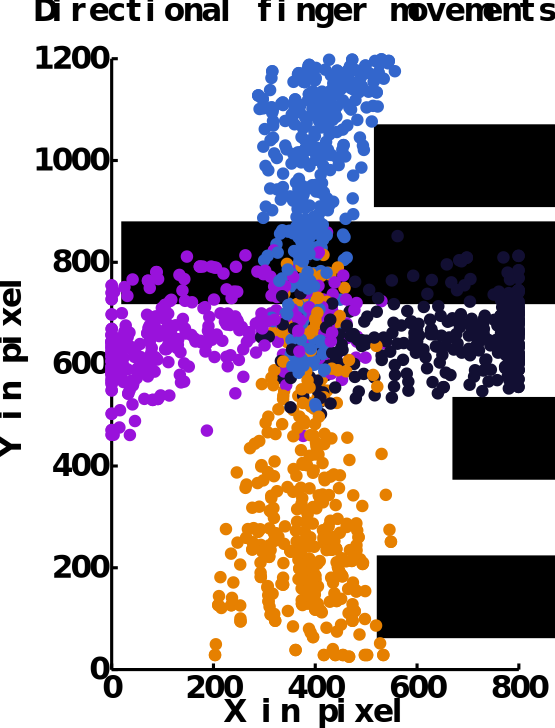
\includegraphics[width=\signalwidth\columnwidth]{\visualspdf/worlds_and_datasets/finger_signals_color.pdf}
\caption{N}
\label{fig:fingerdatasetdirection}
\end{figure} 

Our second dataset shown in Figure~\ref{fig:fingerdatasetsigns} is build from a user drawing The cardinal letters (N, S, W, and E) in the middle of the tablet.

\begin{figure}[!ht]
\centering
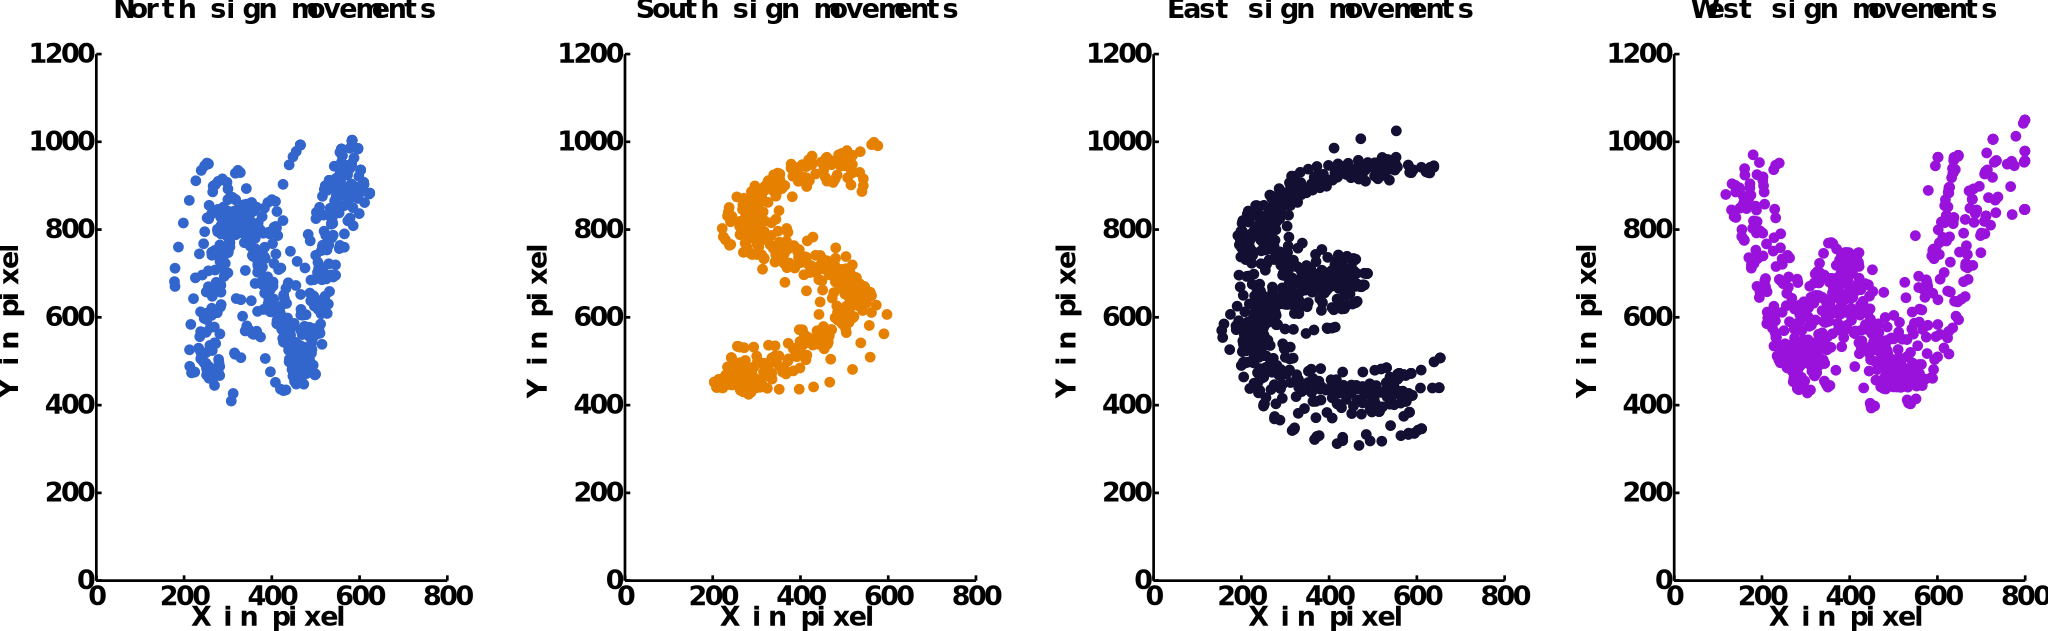
\includegraphics[width=\columnwidth]{\visualspdf/worlds_and_datasets/finger_signals_color_signs.pdf}
\caption{N}
\label{fig:fingerdatasetsigns}
\end{figure} 

To represent those trajectories, our feature vector is composed of 11 dimensions, where dimensions encodes:
\begin{itemize}
   \item The start X and Y positions (2 features)
   \item The end X and Y positions (2 features)
   \item The delta position between start and end position for X and Y coordinate (2 features)
   \item The median X and Y positions (2 features)
   \item The distance between start and end position (1 feature)
   \item The total distance traveled by the finger (1 feature)
   \item The average speed of the finger (1 feature)
\end{itemize}

Using this representation we achieve 100 percent accuracy on the directional movements dataset and 99 percent accuracy on the cardinal signs dataset, using a simple Gaussian classifier with one Gaussian per class.

We remind that the direction of shape of each movement has no a priori meaning for the robot. For example, in our simulation we may use the ``W'' sign signals to mean the goal state is north to the agent position.


\subsection{Evaluating task likelihood}

As there is an infinity of possible goal state, the agent can not estimate the probability of all possible task in parallel. Therefore we will sample a finite number of task at each step and compute a likelihood value for each of those task. Then, given the ranking between them, we will keep some of the best one and sample a bunch of new ones, more details are provided in next subsection~\ref{chapter:limitations:continoushypothesis:particlefilter}.

Our algorithm, as presented so far, was cumulatively accumulating evidence for each task and updated the likelihood of each task on a step by step basis. However for this experiment, as we the task hypothesis are changing step after step, we can not update the likelihood of each task on a step by step basis, as described in Equation~\ref{eq:matchingfiltercrossvalidation}. This approach allowed us to reduce the computational cost of our algorithm so as to be able to run our experiments in a reasonable amount of time. A possible option would be to use Equation~\ref{eq:matchingcrossvalidation}, but we would have to train a huge amount of classifier each step (100000 classifiers after 200 steps in our experiments).

We selected an other option which rely on sampling different classifier from a meta-classifier, which allow us to generate classifiers at a low computational cost. Then given many classifiers for each task, we will compare the likelihood predicted by those classifiers and rank the task by a statistical test on the classifier evaluation. We describe each step of this process in the following paragraph.

The first step is to compute a ``meta'' model which encodes a distribution of probability on the classifier parameters, i.e. which encodes a probability distribution over the mean and covariance of each class. To do so, and given that we are using multivariate normal distribution, we use a noninformative (Jeffrey's) prior \cite{gelman2003bayesian} to estimate the probability distribution over the means and covariances:

\begin{eqnarray}
p(\mu_l|D) & = & t_{n-d}(\mu| \bar{x}_l, \frac{S_l}{n(n-d)})
\label{eq:jeffreysmean}
\end{eqnarray}

\begin{eqnarray}
p(\Sigma_l|D) & = & IW_{n-1}(\Sigma_l | S_l)
\label{eq:jeffreyscov}
\end{eqnarray}

where $\bar{x}_l$ and $\S_l$ respectively represents the ML estimates of the mean and covariance for each class $l$ based on the dataset $D$, $n$ is the number of signals, and $d$ is the dimensionality of a signal feature vector.
$\mu_l$ and $\Sigma_l$ are the posterior probability estimate of the mean and covariance given the noninformative prior. $IW$ denotes an Inverse Wishart function which is the multidimensional generalization of the inverse Gamma, it represents a probability distribution on covariance matrix.

This ``meta'' model encodes the distribution of probability on the classifier parameters. Given this model we can sample, for very low computational cost, a multitude of possible QDA classifiers by sampling a mean and covariance for each class. And the more we have data to fit our model, the less uncertainty remains and the less variability will be observed in the generated classifiers. In our experiment we will sampled 20 classifiers per task.

\todo{text here}


Note that it would seem more straightforward to directly compute the marginal probability distribution of Equation~\ref{eq:prior} which integrates over the all distribution of parameters; and use this for our likelihood estimates of Equation~\ref{eq:matchingoverfitting}. Here we tried to get a measure of confidence on top of our likelihood estimates. This is why we generate several classifiers, test their performances and measure the probability that one set of classifiers is on average better that an other set of classifiers. To do so we model the distribution of performances of a set of classifiers by a normal distribution; and compute the probability that a sample drawn from the distribution associated to one set of classifiers has higher value than one drawn from the distribution associated the an other set of classifiers.

\subsection{Task hypothesis selection and generation}
\label{chapter:limitations:continoushypothesis:particlefilter}

As there is an infinity of possible goal state, the agent can not estimate the probability of all possible task in parallel. Therefore, as described in previous subsection, we sample a finite number of task at each step and compute a confidence measure for each of those task. Given the ranking between them, we will keep some of the best one and sample a bunch of new ones.

\todo{cite particle filtrer}

There is many parameters that will influence the performance of such an algorithm. We can change the number of task sampled, the criteria for selecting the task(s) that stay in the pool from one step to another, and we can change the method used to sample new task. 

As this is an exploratory experiment, we will restrict our analysis to the influence of the method used to resample the pool of task hypothesis and consider either a random or an active strategy. In practice, we will consider a pool of 50 hypothesis. Each step, we will keep the best hypothesis from the pool and replace the 49 others using one of the sampling strategies define next.

The random generation of task simply keeps the best hypothesis and generate 49 new tasks hypothesis randomly.

Our active task generation method simply selects new task around the current best task hypothesis. To do so, we create a mixture of Gaussians which define the probability distribution used to sample the new tasks. This mixture model is composed of:
\begin{itemize}
\item  one fixed Gaussian at the center of the state space (i.e. $[0.5, 0.5]$), with a diagonal covariance matrix, where each value on the diagonal is equal to $0.1$, and have an associated weight of $0.2$. This Gaussian, which as quite spread covariance matrix, maintains a level of exploration in the task generation process.
\item a multitude of Gaussians, one at each location of the previous hypothesis positions (i.e. hypothesized task), whose associated weights are proportional to the probability associated to each task. The sum of the weights of those Gaussians behind 0.8, such as the sum of all mixture component weight is 1. All those Gaussians have a diagonal covariance matrix, where each value on the diagonal is equal to $0.01$. For computational purpose, each Gaussian had a minimal weight of $1e^{-6}$.
\end{itemize}
Note that the resulting distribution will be truncated as all the point generated outside of the boundaries of the space (i.e. between 0 and 1 for each dimension) will be translated to the closest position on the boundaries of the state space.


\subsection{Uncertainty based state sampling}

The agent can also control the next state to teleport to. As seen in chapter~\ref{chapter:planning}, actively controlling agent state important can lead to better performances. Indeed the state of the agent influences the signal sent by the teacher. 

We will compare two kind of active sampling, random and an uncertainty based method. The random method simply teleport the agent to a random position in the world. 

The active method rely again on a sampling method. At each step, we generate 1000 states randomly and compute the uncertainty associated to those states using the method describe in chapter~\ref{chapter:planning} by Equation~\ref{eq:planning} and using up to 20 sampled signals from our history of interaction. For the next state, we select, among the 1000 points, the one that as higher uncertainty, and teleport the agent to that state in order to collect the next teaching signal.


\subsection{Results}

We will compare all four combinations of the methods described above \begin{inparaenum}[a)] \item random state and task selection (which we call ``random random''), \item random selection of next state and active task sampling (which we call ``random active''), \item uncertainty based selection of next state and random task selection (which we call ``uncertainty random''), and \item uncertainty based selection of next state and active task sampling (which we call ``uncertainty active''). \end{inparaenum}

We ran 100 simulated experiments for each method and each dataset. Each experiment lasted 200 iteration and started by 12 random steps such as to collect enough point to use Equation~\ref{eq:jeffreysmean}~and~\ref{eq:jeffreyscov} with our 11 dimensional signals.

\paragraph{Distance to goal state}

For each method, we compare the evolution of the distance between the best task hypothesis through iteration (the more probable according to our estimate) and the goal state (see Figure~\ref{fig:continuoustaskdistevolution}).

\begin{figure}[!ht]
\centering
\includegraphics[width=0.62\columnwidth]{\imgpath/continuous_task/distEvolution.eps}
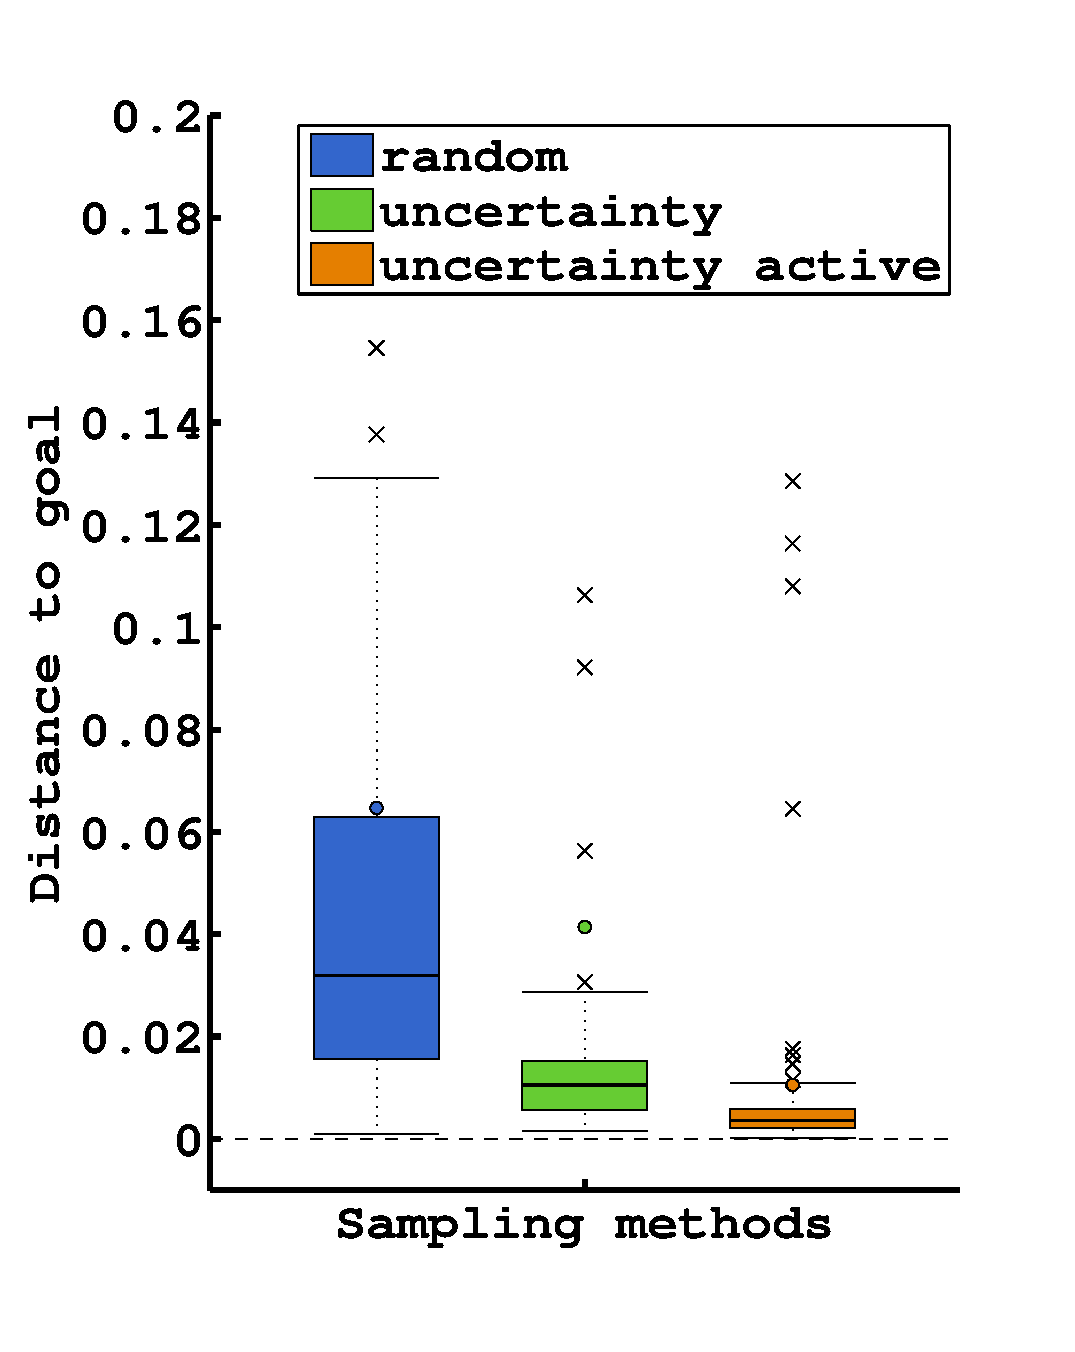
\includegraphics[width=0.37\columnwidth]{\imgpath/continuous_task/endDist.eps}
\caption{Evolution of the distance to target using the directional finger movement dataset shown in Figure~\ref{fig:fingerdatasetdirection}. On the left is the evolution of the distance of the best position hypothesis to the goal position (mean and standard error shown as shaded area). On the right is a box plot of the distance of the best position hypothesis to the goal position at the end of the 200 iterations. Actively sampling new task hypothesis as well as selecting new state based on our uncertainty estimation outperform allow to identify the target position with very high accuracy and low variance. Note that some distant outliers are not shown on the box plots for readability reasons.}
\label{fig:continuoustaskdistevolution}
\end{figure}

Only the combination of actively sampling new task and actively selecting new state based on their relative uncertainty as overall better performance than any other combination of our method. Those two method are complementary, to find a task hypothesis better than our previous best estimates, it is likely that it is close to the current best hypothesis. Our active task sampling method allow to explore close to our previous best estimates. However, now that we have some hypothesis located in a restricted area of the space, we need to sample state in very precise location to be able to differentiate them, which our uncertainty based state selection allow. This explain why using one of the two method alone do not reach the same performances as their combination.

In Figure~\ref{fig:continuoustaskdistevolution} left, we compare the distribution of final distance between our best hypothesis and the true goal position. First note that the important difference between displaying our results in terms of mean and standard error or in terms of a box plot, which shows the median and the 25th and 75th percentile (you can see the mean value as a colored dot). Especially for the ``uncertainty random'' method, the visual impression of the performance of the methods differs. This is due to the outliers, where even a few values far away from the main group of point can ``push'' the mean away, the normal distribution assumption do not hold for presenting our results. In order to statistically compare the efficiency of our methods, we use the Mann-Whitney U-test \cite{mann1947test} which is a nonparametric test for equality of population medians of two independent samples. We will use the one tailed version to specifically test whether one population has greater performances than the other. There is no measurable statistical difference between the ``random random'' and ``random active'' methods ($p = 0.68$). The ``uncertainty random'' performances over ``random random'' ($p<1e^{-10}$) and ``random active'' ($p<1e^{-10}$) are highly significant. As well as the difference between the ``uncertainty active'' and ``uncertainty random'' difference in performance ($p<1e^{-10}$).

The results presented above where obtained using the directional finger movement dataset shown in Figure~\ref{fig:fingerdatasetdirection}. We now demonstrated how the same algorithm could handle different preferences of user finger gesture for cardinal direction indication. To do so we repeat the experiment wit the cardinal sign dataset of Figure~\ref{fig:fingerdatasetsigns}

\paragraph{Task sampling comparison}

\todo{Show the map of sampled task with sampling versus random} 

\paragraph{State sampling comparison}

\todo{Show the end map of sampled state with sampling versus random} 





%%%%%%%%%%%%%%%%%%%%%%%%%%%%%%%%%%%%%%%%%%%%%%
%%%%%%%%%%%%%%%%%%%%%%%%%%%%%%%%%%%%%%%%%%%%%%
%%%%%%%%%%%%%%%%%%%%%%%%%%%%%%%%%%%%%%%%%%%%%%
%%%%%%%%%%%%%%%%%%%%%%%%%%%%%%%%%%%%%%%%%%%%%%
%%%%%%%%%%%%%%%%%%%%%%%%%%%%%%%%%%%%%%%%%%%%%%
%!TEX root = ../../thesis.tex

\section{Interaction frame hypothesis}
\label{chapter:limitations:framehypothesis}

\question{How to relax the assumption that interaction frame is pre-defined and unique?}

Until now we have assumed that the interaction frame, which specifies the details of the interaction between the human and the machine was known. In this section, we considered the case where multiple interaction frames are defined, but only one of them accounts for the interaction between the human and the machine.

% In this frame only the meaning of the signal was unknown. 

\subsection{Illustrations}

We will use a very simple example to illustrate the problem and show computational results. We consider that the agent lives in the line word as defined in chapter~\ref{chapter:lfui::symmetries}, where the agent has access to the ``no move'' action in order to remove the symmetry problem. The agent knowns it should reach either of the two edges of the world, G1 or G2. And the agent knowns that the teacher is providing either feedback or guidance instructions. To handle this new hidden information we will rely again on our interpretation hypothesis process. This time, one hypothesis will be the combination of one task hypothesis and one frame hypothesis. For our simple example, it results in having four hypotheses.

The result of the labeling process is shown in Figure~\ref{fig:multipleframeexplainedfeedback} for a teacher providing feedback instructions according the task G1. The hypothesis that labels the signals according to the task G1 and the feedback frame is the one whose signal-label pairs match better with the underlying structure of the data. Indeed, for the guidance case, the labeling process for hypothesis G1 is always giving a ``left'' label whether or not the agent is moving away or closer to the target, which allows to differentiate between feedback and guidance cases. To differentiate between G1 and G2, the same principle than the one described in chapter~\ref{chapter:lfui::symmetries} applies.

\begin{figure}[!htbp]
\centering
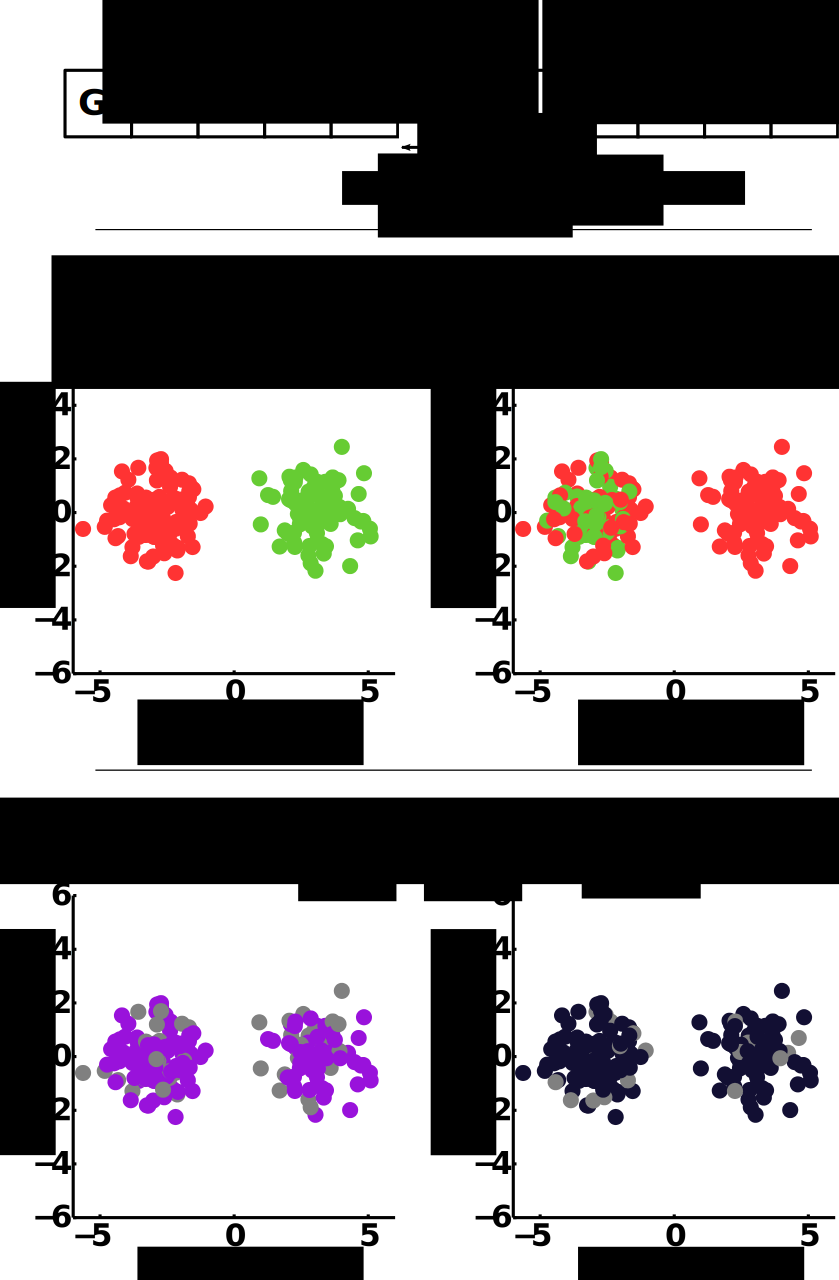
\includegraphics[width=\twoplanningwidth\columnwidth]{\visualspdf/multiple_frame/multiple_frame_feedback.pdf}
\caption{Illustration of the labeling process on both task and interaction frame hypothesis. The agent can perform right, left, or a ``no move'' action. The agent receive feedback on its action in the line word according to G1 . The agent do not known which task (G1 or G2) neither which interaction scheme the teacher is following (feedback or guidance). The result of the labeling process allow to identify the hypothesis on task G1 and feedback frame as the more likely.}
\label{fig:multipleframeexplainedfeedback}
\end{figure} 

Considering now that the teacher is providing guidance instructions according the task G1, the results of the labeling process can be seen in Figure~\ref{fig:multipleframeexplainedguidance}. The same explanation than for Figure~\ref{fig:multipleframeexplainedfeedback} applies. 

\begin{figure}[!htbp]
\centering
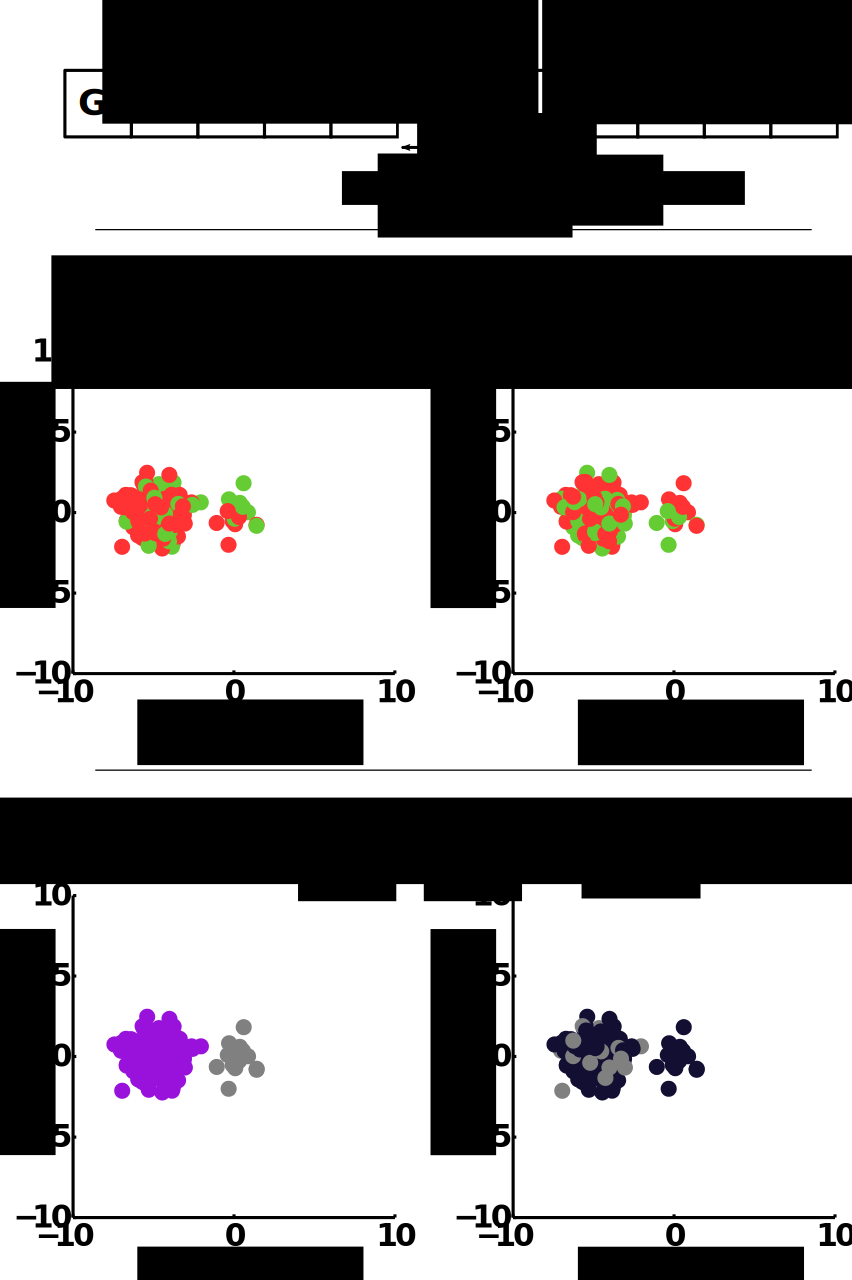
\includegraphics[width=\twoplanningwidth\columnwidth]{\visualspdf/multiple_frame/multiple_frame_guidance.pdf}
\caption{Illustration of the labelling porcess on both task and interaction frame hypothesis. The agent can perform right, left, or a ``no move'' action. The agent receive guidance instruction on its action in the line word according to G1 . The agent do not known which task (G1 or G2) neither which interaction scheme the teacher is following (feedback or guidance). The result of the labeling process allow to identify the hypothesis on task G1 and guidance frame as the more likely.}
\label{fig:multipleframeexplainedguidance}
\end{figure} 

\subsection{Simple experiments}

We now verify that the algorithm works in practice. We consider the same line world scenario as described above. For our experiments, the simulated teacher selects randomly a target (G1 or G2) and an interaction frame (feedback or guidance). The agent is using our uncertainty based planning method. We ran 100 simulations. All other settings were set as for the experiments of chapter~\ref{chapter:planning:method}.

Figure~\ref{fig:multipleframeall} shows the evolution of the probability associated to the correct combination of task and interaction frame (we use the minimum of pairwise normalized likelihood from Equation~\ref{eq:probapairwise} in chapter~\ref{chapter:lfui:confidence}). After 200 steps, all our experiments identified with probability 1 the correct combination of task and interaction frame. 

% In practice, in our previous experiments, we used a confidence threshold of 0.9, under this condition most of our experiments would have identified the task in slighlty more than 50 steps.

\begin{figure}[!htbp]
\centering
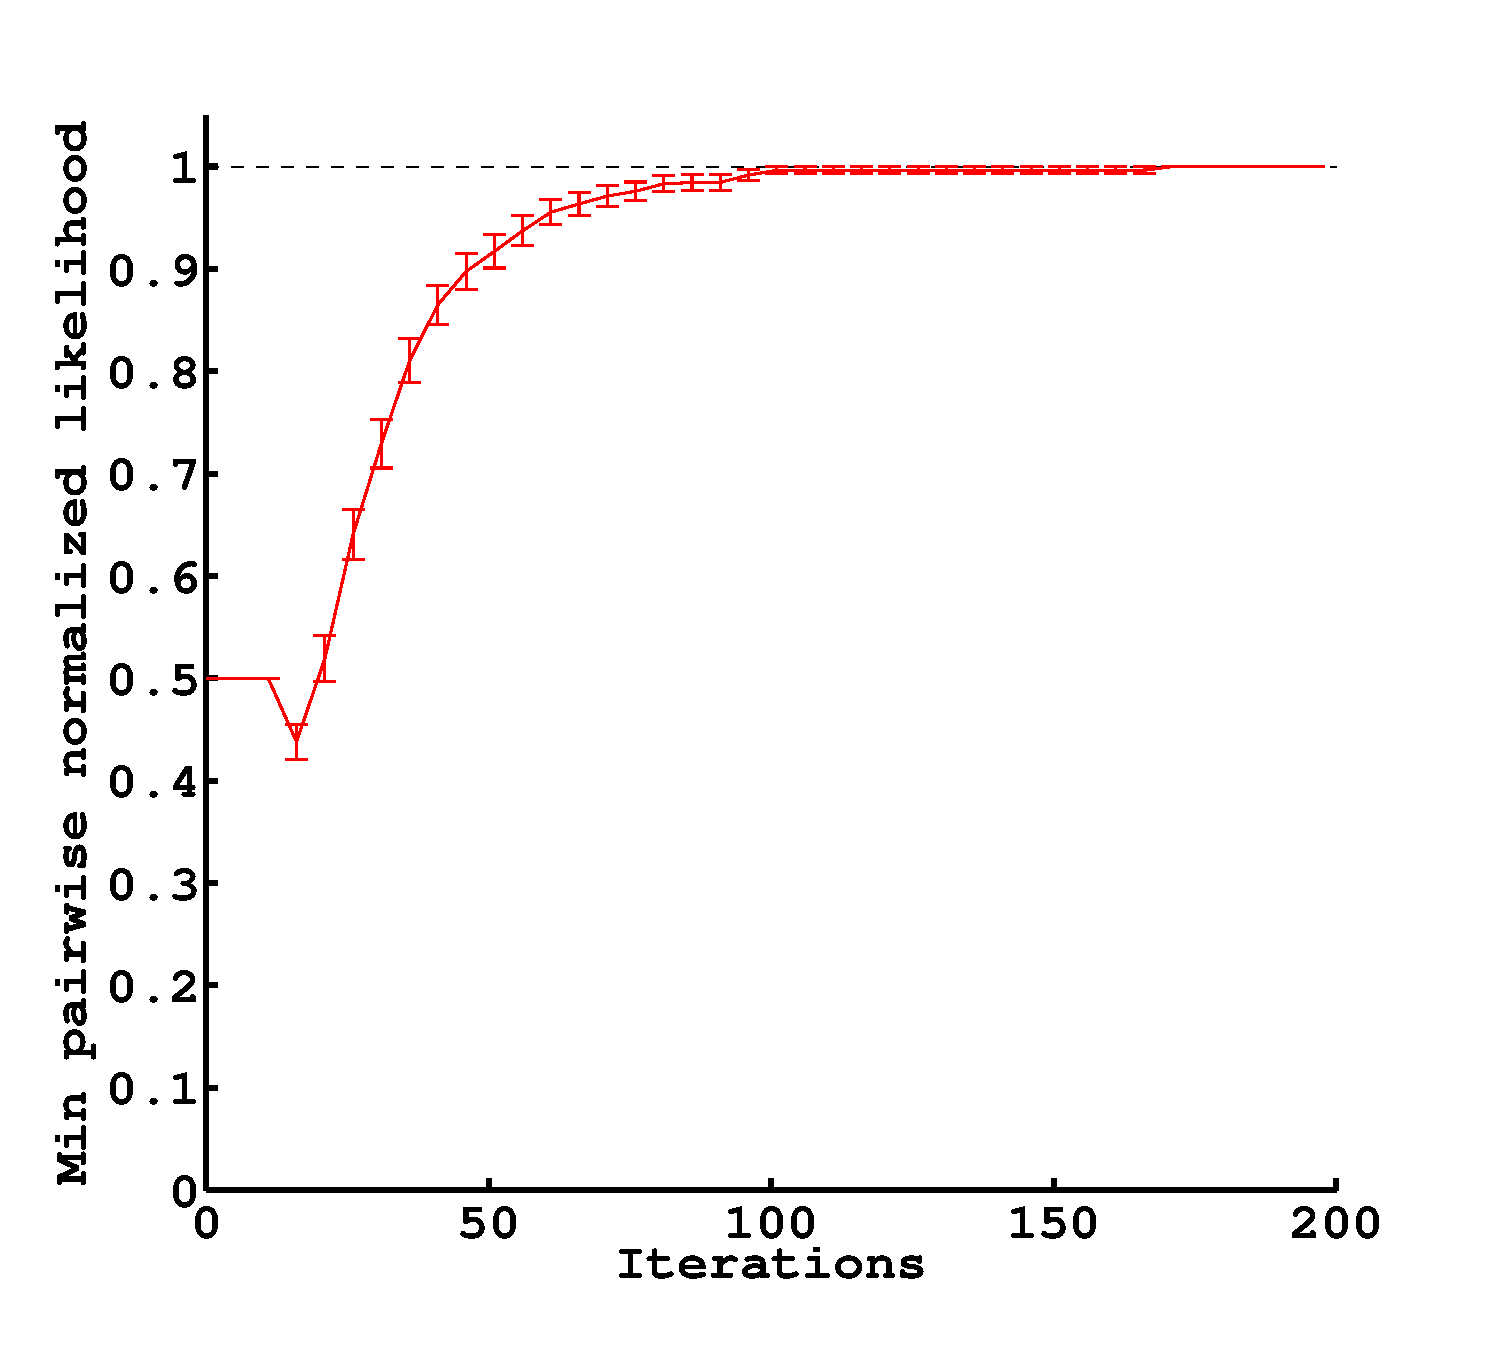
\includegraphics[width=\plotsize\columnwidth]{\imgpath/multiple_frame/multiple_frame_all_teacher.eps}
\caption{Evolution of the minimum of pairwise normalized likelihood for the correct hypothesis. After 200 steps, all our experiments identified with probability 1 the correct combination of task and interaction frame. Most of the experiments would have identified the task slighlty more than 50 steps with a confidence threshold of 0.9.}
\label{fig:multipleframeall}
\end{figure} 

We plot in Figure~\ref{fig:multipleframefeedbackvsguidance} the cases where the teacher was using the feedback frame (left) or the guidance frame (right). The performance are similar in both cases.

\begin{figure}[!htbp]
\centering
\includegraphics[width=0.49\columnwidth]{\imgpath/multiple_frame/multiple_frame_feedback_teacher.eps}
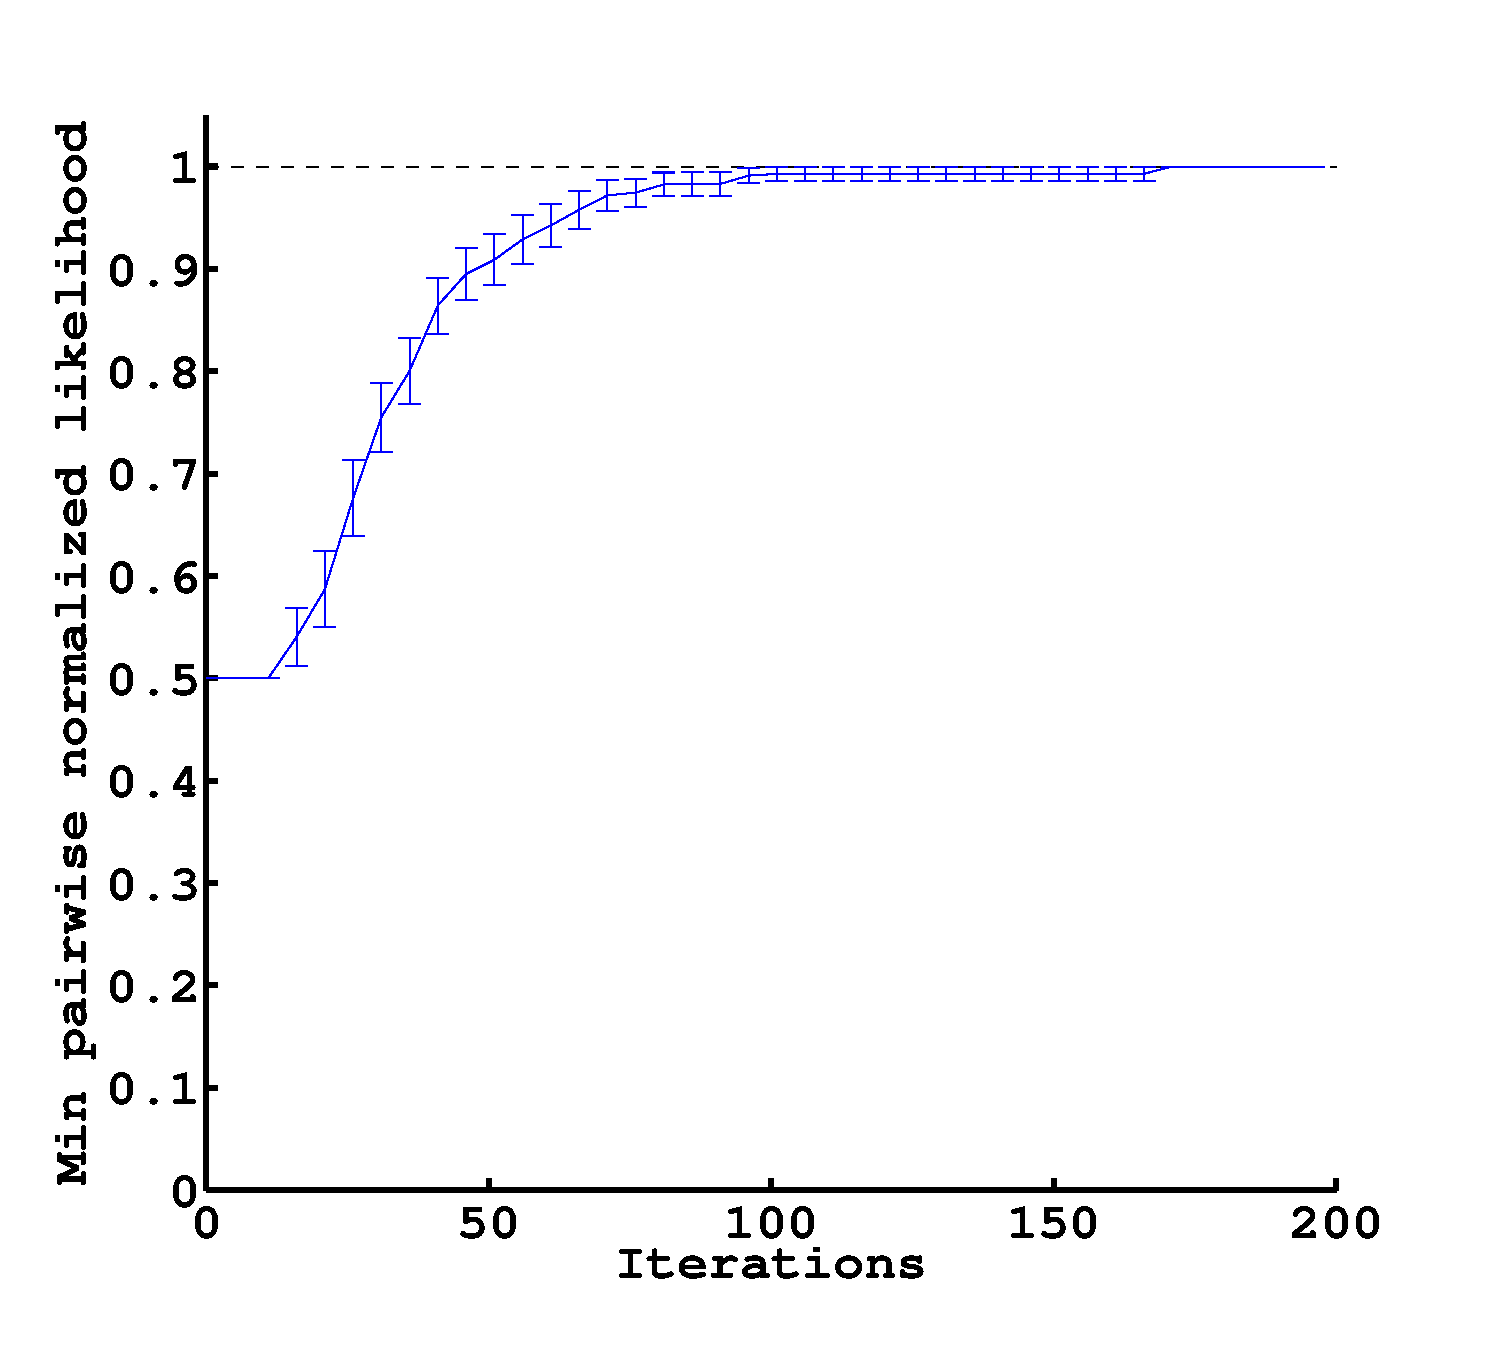
\includegraphics[width=0.49\columnwidth]{\imgpath/multiple_frame/multiple_frame_guidance_teacher.eps}
\caption{Evolution of the minimum of pairwise normalized likelihood for the correct hypothesis if the teacher provided feedback (left) or guidance (right) instruction. After 200 steps, all our experiments identified with probability 1 the correct combination of task and interaction frame. Most of the experiments would have identified the task in slightly more than 50 steps with a confidence threshold of 0.9.}
\label{fig:multipleframefeedbackvsguidance}
\end{figure} 


\subsection{Discussion}

Following the interpretation hypothesis method on a combination of task and interaction frame, we can start learning a task from unlabeled instructions and undefined interaction frames. In other words, such system can not only learn the task and the signal to meaning mapping, but also the interaction protocol used by the teacher.

Considering our example in section~\ref{chapter:limitation:continuoushypothesis}, an application this method can be to consider different coordinate system for the cardinal frame. For example, the signals from the teacher can be relative to the true North magnetic pole, to the current position of the user relative to the agent, or relative to the current orientation of the robot. This experiment performed with a real robot, real users, considering a tablet, and different interaction frames has great potential to demonstrate the potential application of this work.

Finally, we note that a particle filter based method (as used in section~\ref{chapter:limitations:continoushypothesis} for dealing with continuous task) could be considered for dealing with a continuous set of interaction frames. For example, in our example of section~\ref{chapter:limitations:continousstate}, we used a parameterized frame that merged feedback and guidance frame (see Equation~\ref{eq:mixedfeedbackguidance}), and introduced a feedback to guidance ratio $\alpha$. By generating, testing, and resampling a set of $\alpha$, i.e. a set of interaction frames, we may be able to learn, not only the task and the signal to meaning mapping, but also the details of the interaction protocol used by the teacher.

 % For example, in the experiment of section~\ref{chapter:limitations:continousstate} we may identify automatically the $\beta$ parameter of Equation~\ref{eq:mixedfeedbackguidance}.


%%%%%%%%%%%%%%%%%%%%%%%%%%%%%%%%%%%%%%%%%%%%%%
%%%%%%%%%%%%%%%%%%%%%%%%%%%%%%%%%%%%%%%%%%%%%%
%%%%%%%%%%%%%%%%%%%%%%%%%%%%%%%%%%%%%%%%%%%%%%
%%%%%%%%%%%%%%%%%%%%%%%%%%%%%%%%%%%%%%%%%%%%%%
%%%%%%%%%%%%%%%%%%%%%%%%%%%%%%%%%%%%%%%%%%%%%%
\section{Human in the loop}

In real-world applications, users are usually told how to interact with machines. Do people want to have an open-ended choice about what signal to use? Would they be more efficient? When is it better to use a calibration procedure?

how does the agent behavior affect the algorithm assumption on human behavior

Assumption: The properties of the signals do not change wrt. the behavior of the agent

Users comply with the frame implemented. Same meaning, optimal strategies, timing...

discuss how the setup can be used in HRI, but also semiotic stuff...

\paragraph{Usability and user studies}

Only prerecorded datasets have been used. However, signals may change during the learning. For instance, people can try to adapt themselves to a robot if they believe the latter is not understanding properly. Or, brain signals are sensitive to the protocol, the duration of the experiment or even the percentage of errors made by the agent \cite{chavarriaga2010learning}. To which extend the behavior of our agent changes the properties of the teaching signal? Can we adapt to such changes online? 

As we argued in the introduction, the work we presented is a starting point towards forms of adaptive interaction with non-technical users, that we may call fluid interaction learning. While we studied in this article properties of learning algorithms that will be needed for such an endeavor, it remains to be shown how they can be integrated within a full real-world human-robot interaction scenario and architecture so that the usability and acceptability of such system can be evaluated. Thus, user studies in particular will be a crucial next step of this work. Some improvements of the system may be needed to reach acceptable levels of usability.
Indeed, our current system can be restrictive for the user as the number of interaction increases quickly with the complexity of the size of the task and meaning spaces. However, we have shown that the system is able to use known sources of information, which in real-world interaction could be leveraged to keep the sample complexity low.

In relation to targeting fluid interaction learning, we will consider in the future how more complex kinds of instructions can be included in our formalism. Indeed, the possible teaching models used spontaneously by people can be more complex than the simple meaning correspondences we assumed \cite{thomaz2008teachable,Cakmak2010optimality}. Also the turn taking scheme could be made more natural, as the robot could ask questions \cite{cakmak2012designing} and accept asynchronous instructions.

%%%%%%%%%%%%%%%%%%%%%%%%%%%%%%%%%%%%%%%%%%%%%%
%%%%%%%%%%%%%%%%%%%%%%%%%%%%%%%%%%%%%%%%%%%%%%
%%%%%%%%%%%%%%%%%%%%%%%%%%%%%%%%%%%%%%%%%%%%%%
%%%%%%%%%%%%%%%%%%%%%%%%%%%%%%%%%%%%%%%%%%%%%%
%%%%%%%%%%%%%%%%%%%%%%%%%%%%%%%%%%%%%%%%%%%%%%
\section{Word properties}
xp with a grid world versus a real maze with many wall and see that random becomes a joke

\paragraph{Symmetric task repertoires} Our approach assumes that the robot is equipped with planning skills and can not be used if several hypothesis are fully symmetric as they will not be differentiable. This latter problem can be solved by redefining the set of hypothesis, for instance by adding a ``stop'' action valid only at the goal states.

How the task properties (symmetries, size, \ldots) affect the learning properties?




%%%%%%%%%%%%%%%%%%%%%%%%%%%%%%%%%%%%%%%%%%%%%%
%%%%%%%%%%%%%%%%%%%%%%%%%%%%%%%%%%%%%%%%%%%%%%
%%%%%%%%%%%%%%%%%%%%%%%%%%%%%%%%%%%%%%%%%%%%%%
%%%%%%%%%%%%%%%%%%%%%%%%%%%%%%%%%%%%%%%%%%%%%%
%%%%%%%%%%%%%%%%%%%%%%%%%%%%%%%%%%%%%%%%%%%%%%
\section{A minimalist proof}

proof and more simple scenario to analyse in more details what is happening and the porperties of this work is defninitevely missing and was not my principal interrest when develloping this work. As everyone as its prefered skills, I am sure there will be interrest people to work on this.

lack of proof

\subsection{Interpretation hypothesis: a symbolic signal example}

We further assume that the user is coherent and uses one signal for one meaning. The assumption is that the mapping between symbolic signals and their meaning can only be of two forms.

It could be exemplified by an interface with two buttons, one for ``correct'' and one for ``incorrect'', but the mapping between the button and the meaning would not be defined in advance.

\todo{figure with possible mapping}

For a particular hypothesis, the robot can assign hypothetic meanings)to the human signals knowing their are limited to a fixed set and according to the current state of the world. The machine is ``reasoning'' as follow: \emph{"If the human wants me to solve task G1 then when I performed action $a$ in state $a$ and he said ``oui'', he meant ``incorrect''"}. 

\todo{example step by step, first the world, one action, it interpretation wrt. each hypothesis, then accelerate and observe}

By creating a set of hypothesis, the system end-up with a set of possible interpretation of the human teaching signals. But as the user have only one objective in mind, here G1, only the correct interpretation will exhibit a coherence between the signals and their associated meanings. 

In our case, as the user is using symbolic signals, and that we assumed the user is coherent and use always the same symbol for the same meaning. We can infer that hypothesis G1 is the correct one as the resulting mapping between signal and meaning is more coherent.

\todo{For the symbolic case, and given specific constraint we will present a minimalist proof once the associated mathematical notation will be introduced}

The example described above simplifies the problem in some aspects. Indeed we assume the robot is already able to discriminate between perceptual events and has access to a unlabeled symbolic representation of the teaching signals. It would be the case when using a button based interface, however, when considering more ``natural'' means of interaction such as speech, the mapping between spoken words and their meaning should be learn by the machine. Indeed, the same word in never pronounced exactly the same way and some classification algorithm should be applied to train a discriminative model.


\section{stuff}

\subsection{Coherent means nothing}

Similarly, the system assumed a pre-defined repertoire of possible meanings to be associated with continuous instruction signals. Extending the system towards the creation of novel meanings is an important question. Another approach, for both extending task and meaning repertoires dynamically, would be to allow the user to teach the robot new macro-actions, associated to new macro-instructions, or macro-state, for example based on the options framework \cite{sutton1999between}.

The space of tasks to be sampled at a given moment may also be constrained by the current situation and context (for example, a robot hearing the instructions of a human while he is looking at cubes on a table may infer that the task has a higher probability to be defined in terms of manipulation of these cubes than to change the state of an object in another room). 